\documentclass[11pt,a4paper,twoside,openright]{scrbook}
\usepackage{clba}
\usepackage{hyperref}
\usepackage{natbib}
\usepackage{tabularx}
\usepackage{subcaption}

% Per Kapitel Nummerierung von Graphiken und Tabellen
\usepackage{chngcntr}
\counterwithin{figure}{chapter}
\counterwithin{table}{chapter}


% Hier die eigenen Daten eintragen
\global\fach{Computerlinguistik}
\global\arbeit{Bachelorarbeit}
\global\titel{Evaluating Character-Level Recurrent Neural Networks}
\global\bearbeiter{Leonie Weißweiler}
\global\betreuer{Prof. Anna Korhonen}
\global\pruefer{Prof. Alexander Fraser}
\global\universitaet{Ludwig-Maximilians-Universität München}
\global\fakultaet{Fakultät für Sprach- und Literaturwissenschaften}
\global\department{Department 2}

\global\abgabetermin{28. Mai 2018}
\global\bearbeitungszeit{19. März - 28. Mai 2012}
\global\ort{München}


\begin{document}

% Deckblatt
\deckblatt

\pagestyle{scrheadings}
\pagenumbering{gobble}

% Erklärung fürs Prüfungsamt
\erklaerung

% Zusammenfassung
\addchap{Abstract}
\thispagestyle{scrplain}
\noindent
Character-level recurrent neural networks are a promising new direction for language modelling as they can capture character-level dependencies and thereby learn about morphology, something that word-level models are unable to do. However, using them bears the risk of the models producing output that does not consist of actual words. In order to assess the usability and current progress of word-level recurrent neural networks, we develop evaluation criteria for quantifying the risks and advantages associated with them. Previously, the networks had mainly been evaluated using Perplexity, which does not capture the concrete disadvantages and advantages of character-level models well. The criteria are the correctness percentage, which measures what percentage of the output of the model consists of correct words, and the new sensible word count, which measures how many correct words were newly generated by the model. We then evaluate four kinds of recurrent neural networks on 38 languages. We find that the correctness percentages generally range between 70\% and 80\%, and that a cell found by Neural Architecture Search and Gated Recurrent Units perform better regarding correctness percentages, while simple Recurrent Neural Networks and Long-Short-Term Memory Networks perform better regarding the new sensible word count. 

% Inhaltsverzeichnis
\pagenumbering{Roman}

\tableofcontents

% Text mit arabischer Nummerierung
\pagenumbering{arabic}

\chapter{Introduction}
Character-level models form an important part of language modelling, as they can do something that word level models cannot: namely, learning about and modelling not only relations between words but also the relations between characters within individual words. Additionally, they are not reliant on pre-processing steps such as tokenisation. This means they are in principle superior to word-level models, as they can model more aspects of languages. However, they attract a major risk which word-level models do not: it is possible for them to produce gibberish as output, rather than words. As a result, character-level models are not universally used, despite their potential advantage over word-level models.
Therefore, there are two criteria that someone deciding between character and word-level models for their application must consider. Firstly, to what degree it achieves its goal of modeling character-level dependencies, as otherwise there would be no reason to choose it over a word-level model. Secondly, to what degree it performs worse than a word-level model on account of generating words that do not actually exist. So far, character-level models have mostly been chosen with little regard to these criteria, and evaluated against each other using perplexity scores, which – while scoring how well the model was able to adapt to the data – does not evaluate the model against the criteria that is actually required of it.
This thesis aims to present both innovative and easy-to-compute criteria for evaluating character-level language models, and the first comprehensive evaluation of four kinds of character-level recurrent neural networks trained on 38 languages. We believe that this will be a significant aid for any researchers considering using a character-level network for their work, as we can recommend which kind of character-level network to use for each language. We also answer the two major questions about character-level models: how many non-words they produce, and how well they capture character-level dependencies.
We achieve this by introducing two metrics. The first is the correctness percentage, which is the amount of words that the model has generated that could be found in a large corpus and are therefore assumed to be correct, divided by the total number of generated words. This measures how well the model was able to generate correct words, thus effectively measuring how great the disadvantage is compared to word-level models. The second is the number of new sensible words, which is the number of words generated by the model that have not been observed in the training data, but are found in the large reference corpus. Thus, they are the number of correct words that the model has generated itself, not just repeated, which makes them a measure for how well the model has achieved its original goal of capturing character-level dependencies and having an advantage over word-level models.
We find that for many languages, there is a trade-off between models: the higher they score on the correctness percentage, the fewer new sensible words they generate, and vice versa. This means that the choice of model depends priorities of the application and user. However, for many other languages, either LSTM works better, or NAS better than GRU, or both. This means that while the trade-off is still present, some models are superior to others in both metrics. We also find that the better the correctness percentage, the closer the type token ratio is to that of the original data, which implies that it might be possible to use type token ratio analysis as a first indicator of model performance. We also find that agglutinative and isolating languages perform better than average across all models. 
The remainder of this thesis is structured as follows. Chapter 2 is dedicated to the technical and linguistic background. Chapter 3 presents the related work. Chapter 4 details the methods used for measuring performance further. Chapter 5 details the datasets and evaluation setup used. Chapter 6 presents and analyses the evaluation results. Overarching conclusions are summarised in chapter 7.


\chapter{Background}

\section{Machine Learning Background}
\subsection{Language Modeling}
A language model is a function that puts a probability measure over the words or characters of any given text. It can take into consideration not only the word or character itself, but also those preceding it.  Once trained, it can assess the probability for a given string to belong to that language – for example, to pick between possible transcriptions generated through optical character recognition or speech-to-text. By repeatedly picking the most probable next symbol or sampling from the probability distribution, language models are also capable of generating text.
\cite{irbook}

\subsection{Recurrent Neural Networks}
\label{section:NNs}
When attempting to model language with neural networks, it is important to consider how well the neural network is able to model sequential data \cite{mikolov}. Regular neural networks that only use the specific information its given to compute the probability of a symbol, also called feed-forward neural networks (FFNNs), as used by \cite{bengio} use contexts of fixed length, which needs to be specified before training. It means that the network can only see a finite amount of preceding words, usually five to ten, when computing the next word. This is not satisfactory as it is obvious that humans can make use of far larger context when speaking.
The solution to this problem are Recurrent Neural Networks, first introduced by \cite{elman}. Recurrent Neural Networks are a family or class of neural networks designed for processing sequential data and generating new sequences \cite{goodfellow}. They can scale to much longer sequences than would be practical for FFNNs and are able to process sequences of variable length. Four kinds of neural networks will be used in this thesis and discussed here: simple recurrent neural networks, long-short-term memory networks, neural architecture search and gated recurrent unit network.

\subsubsection{Simple Recurrent Neural Networks}

\begin{figure}
\centering
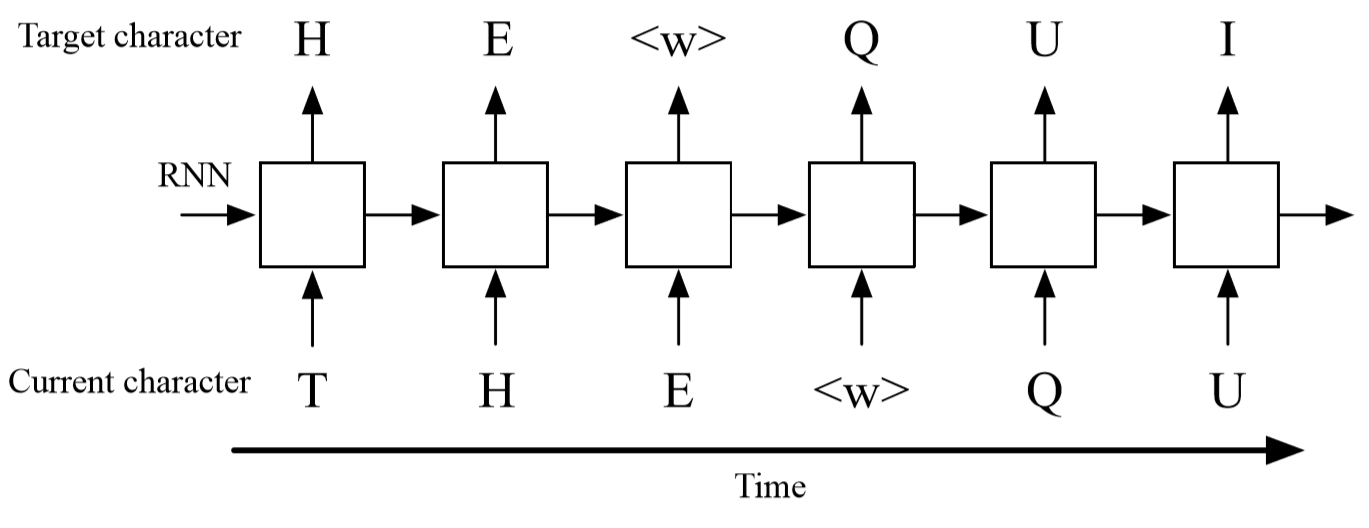
\includegraphics[width=0.7\textwidth]{images/hwan_char_rnn.png}
\caption{A recurrent neural network \cite{hwang}}
\label{Figure:RNN}
\end{figure}

A simple recurrent neural network (RNN), or Elman network, is illustrated in Figure \ref{Figure:RNN}. It operates by passing each element of the input vector sequence $x = (x_1, ..., x_T)$ through a stack of N hidden layers, that each produce a hidden state $h^n_t$ in every timestep, while the last one outputs an output vector $y_t$. Each output vector $y_t$ is used to parameterise a predictive distribution $Pr(x_t+1|y_t)$ over the possible next characters, which are also the next input $x_t+1$. The crucial difference to FFNNs is that in an RNN, each hidden layer does not only receive the hidden state of the layer below as an input, but also its own hidden state from the timestep before. The function evaluated to calculate a layer’s hidden state is therefore the same as for a regular neural network, with the difference that that the input $x_t$ is augmented by the last hidden state $h_{t-1}$ before being multiplied by the weight matrix:
	
\begin{equation}
h_t = \sigma (W \cdot [x_t, h_{t-1}] + b)
\end{equation} 

This makes it possible for information to remain inside the network for an arbitrarily long time, thus enabling the network to consider, theoretically, an infinitely large context when computing the next output of the sequence. 
Therefore, in an RNN, the hidden state serves a double purpose. In a feedforward network, the hidden units would only develop internal representations for the input patterns; this enables the network to produce an output given some input \cite{elman}.  In an RNN, however, the hidden units are now also tasked with modelling what should be remembered from the last hidden state. At the same time, they are also mapping from the input, the learned patterns, and the previous hidden state to some output. This means that when they are trained, they develop in such a way that they are sensitive to temporal context, as the effect of time is implicitly learned in the hidden states.
An RNN is trained by processing training data sequences one step at a time and predicting the next output, then feeding the generated output as input for the next time step \cite{graves}.

\subsubsection{Long-Short Time Memory Cells}
In theory, the architecture of RNNs should enable them to store information indefinitely. However, there are several problems with this in practice.A new type of RNN layer called Long-\textit{Short-Term Memory Cell} (LSTM) was proposed by \cite{hochreiter-schmidhuber} that solves these problems.
One problem is that a standard RNN is prone to instability, as it cannot store information about past inputs for very long. If the model produces several errors and produces several wrong words when generating, it has little opportunity to recover from its mistakes, as these mistakes are fed back into the network and it cannot make use of earlier, correct information. When the gradient of the error function of the RNN is propagated back through the network, it is scaled by a factor for each unit it passes. This factor is, in most cases, greater or smaller than one. As a result, the error gradient either blows up or decays exponentially over time, which means that it either dominates the next weight adaptation step or is not counted at all. The LSTM unit avoids this effect because the scaling factor is fixed to one\cite{sundermeyer}. \cite{graves}

Essential to the LSTM architecture is that each unit maintains a memory cell received from the same unit at the last timestep, modified and passed along to the same unit at the next timestep. It is also used to calculate the hidden state that is passed on to the next unit in the same timestep. The overall structure is displayed in Figure \ref{Figure:LSTM}.

\begin{figure}
\centering
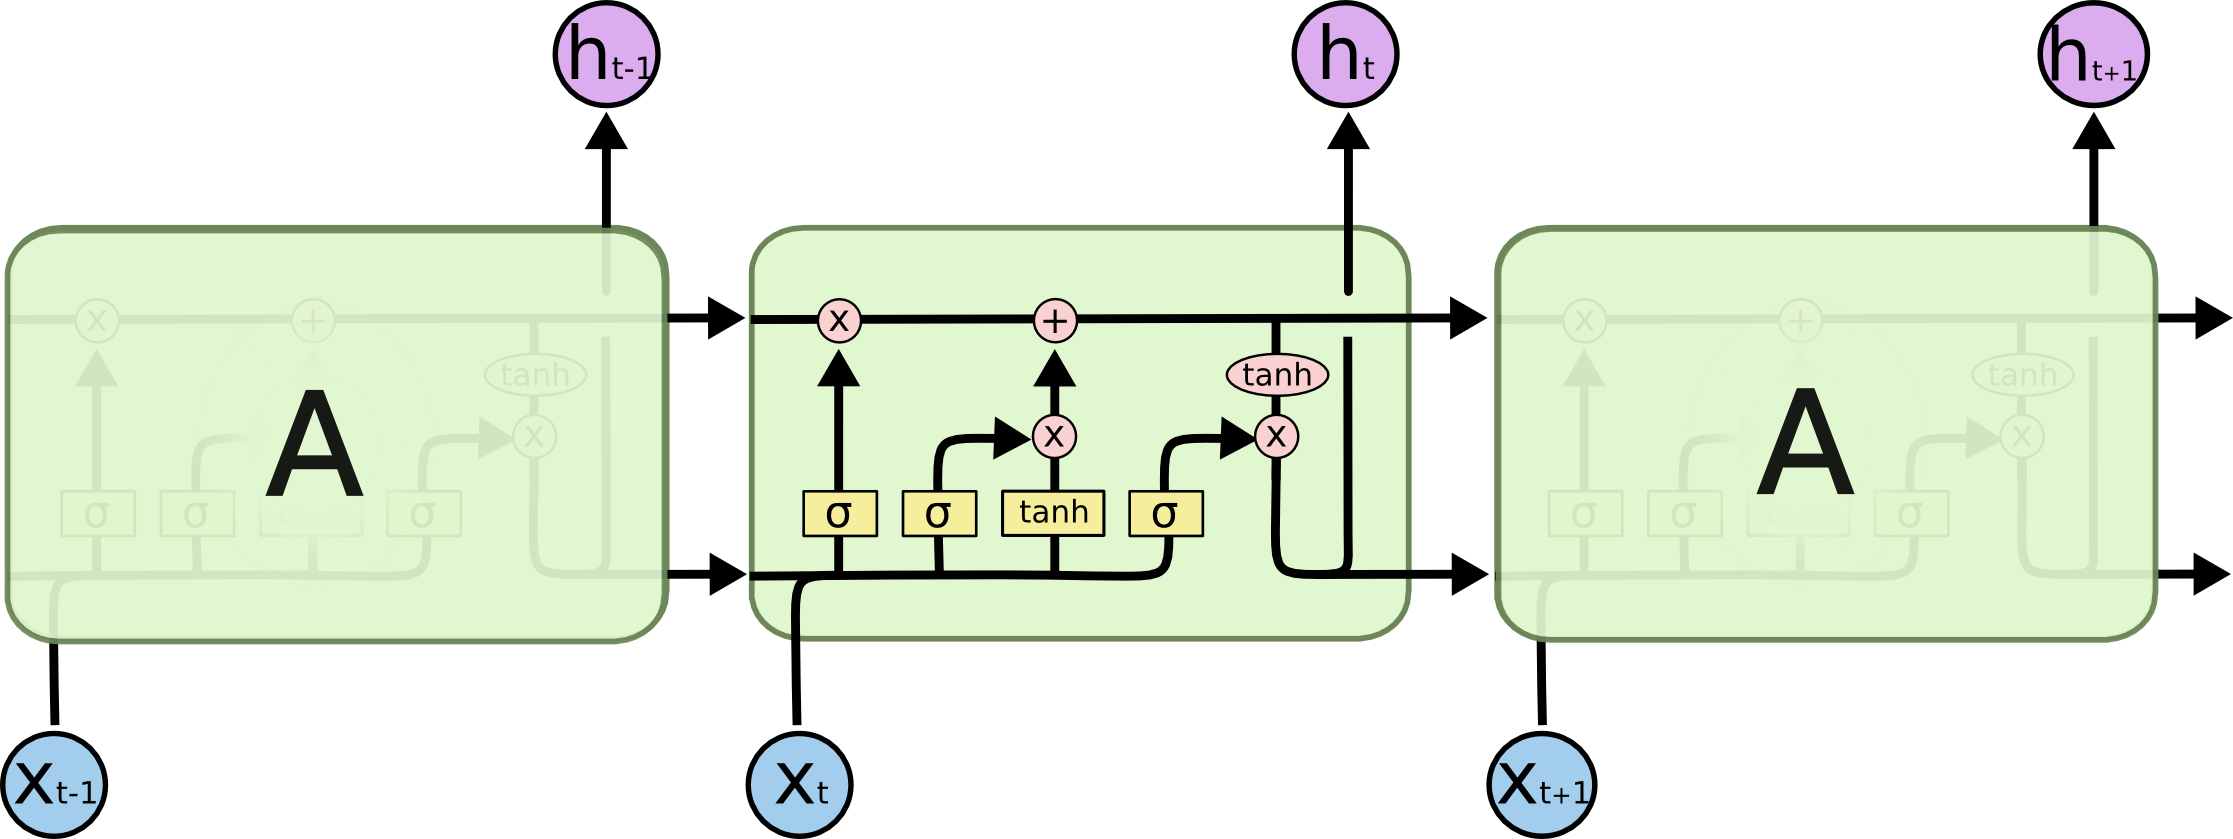
\includegraphics[width=0.9\textwidth]{images/LSTM.png}
\caption{The LSTM cell. \tiny{From \url{http://colah.github.io/posts/2015-08-Understanding-LSTMs/}}}
\label{Figure:LSTM}
\end{figure}

The first modification to the memory cell is made by a sigmoid layer called the “forget gate layer”. It receives both the unit’s input at the current timestep and the hidden state from the last timestep, and computes a value between 0 and 1 for each element of the memory cell using a single neural network layer with a sigmoid activation function:

\begin{equation}
f_t = \sigma (W_f \cdot [h_{t-1},x_t] + b_f)
\end{equation}
	
The memory cell is then element-wise multiplied with $f_t$. This step allows the network to selectively remove data from the memory cell. In the next step, new information is added to the memory cell via the input gate. First, the unit’s input and the last hidden state are fed through a tanh neural network layer to compute a vector of new candidate values $\widetilde C_t$ to be added to the memory cell:

\begin{equation}
\widetilde C_t = \tanh(W_c \cdot [h_{t-1}, x_t] + b_C)
\end{equation}
	
Before the values are added to the memory cell, they are multiplied with the output of another sigmoid neural network layer which selectively reduces some of the candidate values, called the input gate:

\begin{equation}
i_t = \sigma (W_i \cdot [h_{t-1},x_t] + b_i)
\end{equation}
The new memory cell values are then computed from the gate- and candidate values:
\begin{equation}
C_t = f_t \cdot C_{t-1} + i_t \cdot \widetilde C_t
\end{equation}
	
Each element of the new memory cell is then passed through a tanh activation function, and then through the output gate, which computes the output hidden state by using another sigmoid neural network layer’s outputs multiplied with the output values.

\begin{equation}
o_t = \sigma (W_o \cdot [h_{t-1},x_t] + b_o)
\end{equation}

\begin{equation}
h_t = o_t \cdot \tanh(C_t)
\end{equation}

\subsubsection{Gated Recurrent Units}
The Gated Recurrent Unit, GRU, proposed by \cite{cho}, is a variant of LSTM that is simpler to compute and implement. Unlike the LSTM cell, GRU has no separate memory cell. Instead, it uses the hidden state both for transferring information to the next layer in the same timestep as well as to the same layer in the next timestep. Its structure is depicted in \ref{Figure:GRU}.


\begin{figure}
\centering
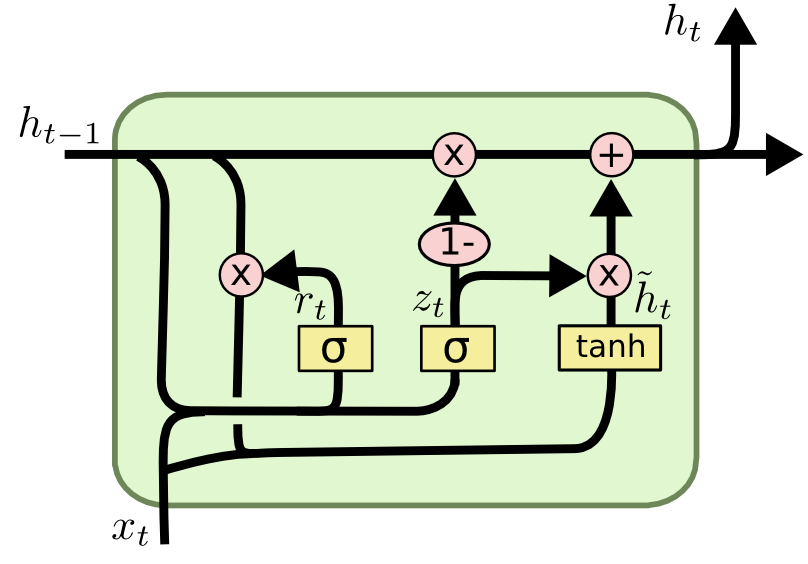
\includegraphics[width=0.5\textwidth]{images/GRU.png}
\caption{The GRU cell. \tiny{From \url{http://colah.github.io/posts/2015-08-Understanding-LSTMs/}}}
\label{Figure:GRU}
\end{figure}

The first gate is the reset gate, which is computed by applying a neural network layer with a sigmoid activation function to the input and the last hidden state:

\begin{equation}
r_t = \sigma (W_r \cdot [h_{t-1},x_t] + b_r)
\end{equation}
	
The output of this gate is then multiplied with the hidden state. Its purpose is to preselect the information from the last hidden state that is relevant to the computation of the update values. To compute these values, the current input and the hidden state that has been modified by the reset gate are passed through neural network layer with a tanh activation function that decides the candidate update values for the new hidden state:

\begin{equation}
\tilde h_t = tanh (W \cdot [(r_t \odot h_{t-1}), x_t] + b )
\end{equation}
	
The update gate takes the previous hidden state and the current input and computes a vector of values between 0 and 1 which decide by how much every value in the hidden state will be updated:

\begin{equation}
z_t = \sigma (W_z \cdot [h_{t-1}, x_t] + b_z)
\end{equation}

Finally, the old hidden state and the candidate update values are summed up, each weighted according to the update gate’s output to produce the hidden state:

\begin{equation}
h_t = (1 - z_t) \cdot h_{t-1} + z_t \cdot \tilde h_t
\end{equation}

There are several differences between LSTM and GRU. Firstly, GRU can only override old information with new information since there is only a single gate that modifies the hidden state, while LSTM features a forget and an update gate, which independently remove and insert information from and to the memory cell. Secondly, because GRU always outputs its full hidden state, it lacks the output gate that allows LSTM to control what part of its memorized information is exposed to the subsequent layers. Finally, the reset gate allows GRU to ignore information from the last hidden state by computing the candidate values, while LSTM always considers both the current input as well as the last hidden state for this procedure.

\subsubsection{Neural Architecture Search}

\begin{figure}
\centering
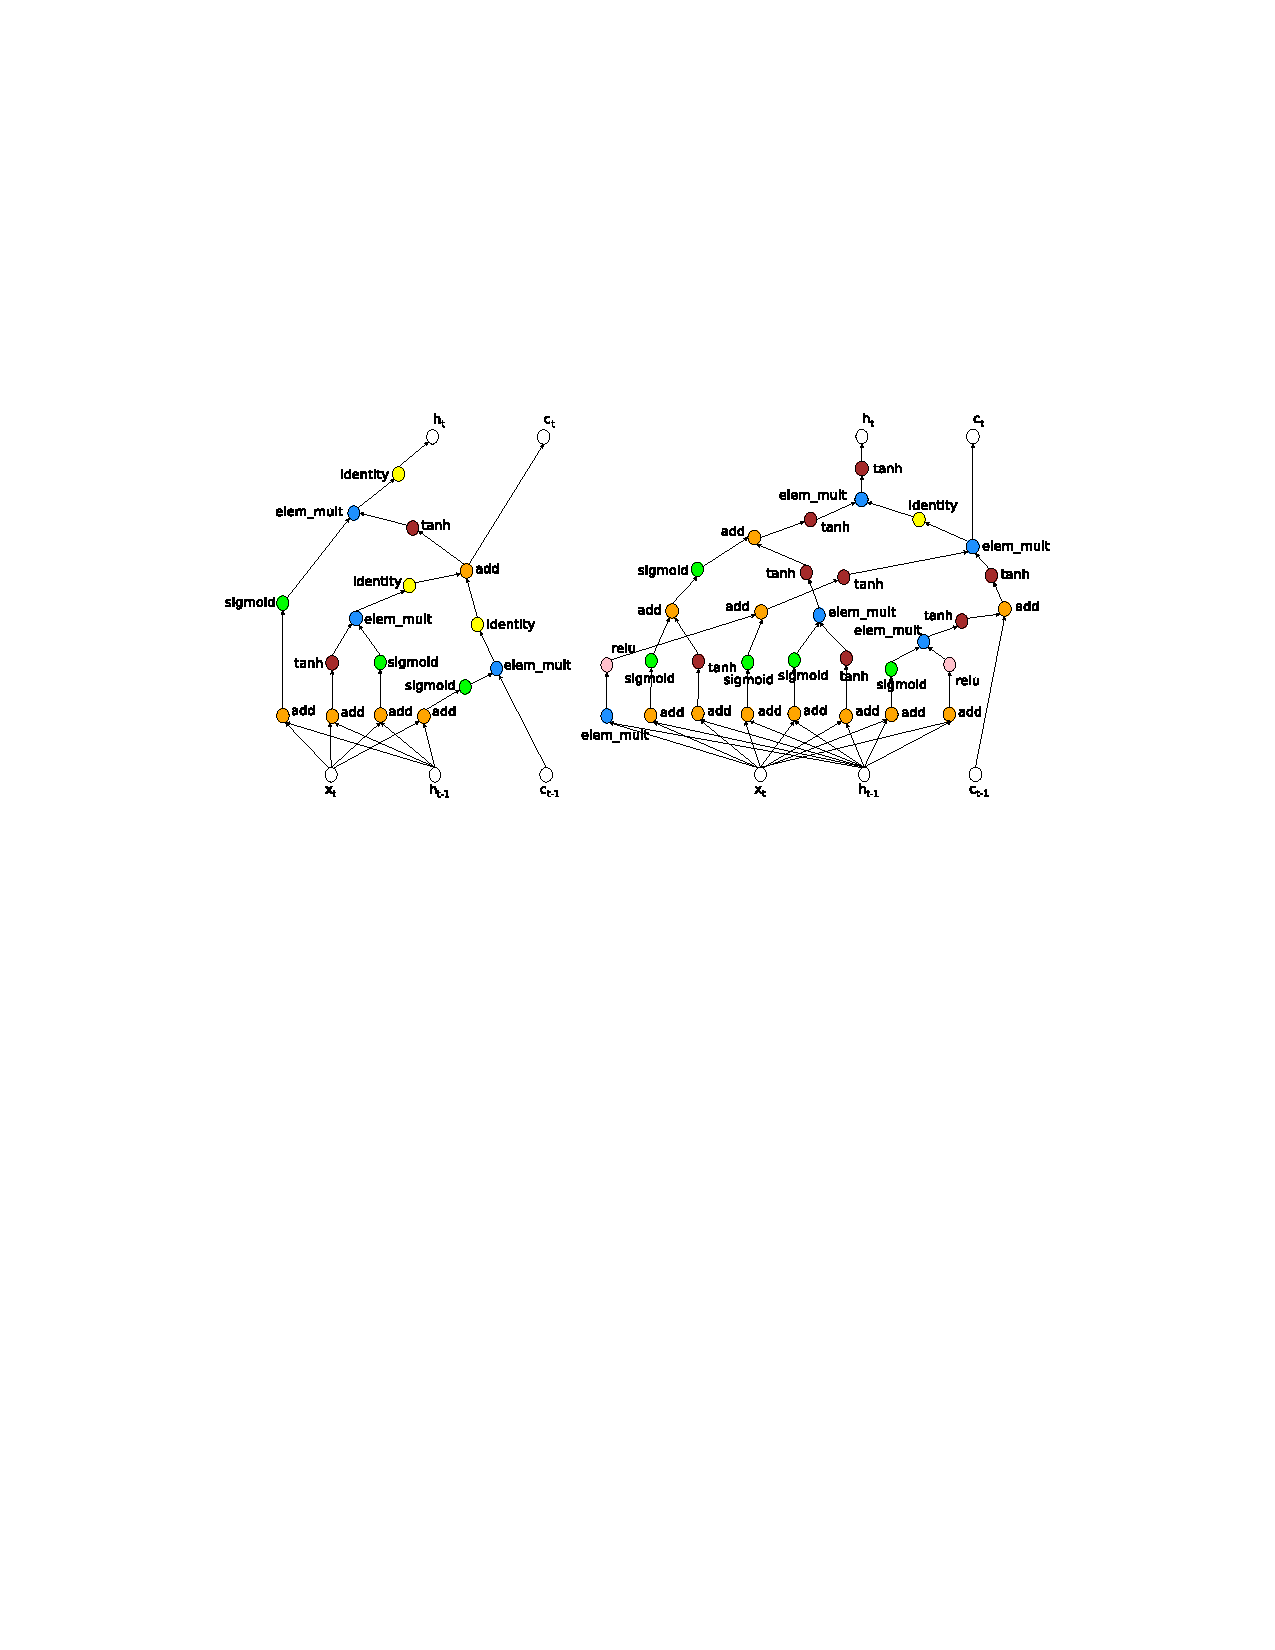
\includegraphics[width=0.8\textwidth]{images/NAS.pdf}
\caption{A LSTM cell on the left, compared to a RNN cell generated using NAS \cite{zoph}}
\label{Figure:NAS}
\end{figure}

Neural Architecture Search (NAS) is a method of finding good network architecture descriptions for a given problem that was introduced by \cite{zoph} in 2016. A controller RNN is used to generate hyperparameter descriptions of neural networks, from which actual networks are generated, trained and evaluated. Their performance is then used to train the controller network using reinforcement learning. Among other experiments, the authors used this method to find an optimal RNN cell by specifying a parameterised general cell and letting the controller network pick operations and activation functions. Each unit generated by the NAS includes a hidden state and a memory cell, similarly to LSTM. One of the specific units they found can be seen in Figure \ref{Figure:NAS}. This is the unit used in this thesis. It has roughly twice as many operations and activation functions as a regular LSTM unit, which is depicted to the left in Figure \ref{Figure:NAS}. The authors performed NAS using different language modelling and machine translation tasks to find the cell. They could not provide any insight into why the network chose this particular architecture or why it might be superior. 

\section{Linguistic Background}
\subsection{Heap's Law}
Heap's law is an empirical law which estimates the vocabulary size of a text as a function of document length: \[ M = kT^b \] where M is the number of types and T the number of tokens in the collection.k and b are parameters that vary with the data, typical values for them being  \( 30 \leq k \leq 100\) and \(b \approx 0.5\) \citep{Heaps} \cite{herdan}

\subsection{Zipf's Law}
Zipf's law formulates the empirical observation that in any sufficiently large corpus, the frequency $f$ of the $i$th most common word is proportional to $\frac{1}{i}$ \cite{irbook}. Intuitively, this means that frequency decreases rapidly with rank, meaning that most words in the corpus occur only once or twice. 

\begin{equation}
f_i \propto \frac{1}{i}
\end{equation}

\subsection{Morphological Typology}
Morphological Typology is the division of languages according to their common morphological structures. The most general divide is between synthetic and isolating languages. Isolating languages allow no affixation at all, so that words consist only of one morpheme. Therefore, only free morphemes exist in isolating languages. Synthetic languages, on the other hand, allow affixation, which means that words may include two or more morphemes. These languages have bound morphemes, which must be attached to another morpheme, in addition to free morphemes. Synthetic languages can be further divided into fusional, agglutinative, and polysynthetic languages. Fusional languages, in addition to their synthetic properties, may have morphemes that combine multiple pieces of grammatical information. As a result, there is no clear 1 to 1 relationship between grammatical information and morphemes. Agglutinative languages have morphemes that are easily parsed, since morpheme boundaries within words are easy to identify. Polysynthetic languages may have words with multiple stems in a single non-compound word. This is achieved, for example, by combining the subject and object nouns into complex verb forms.
\cite{linguistic-typology} \cite{haspelmath}.
For the sake of computational analysis, the typology is often simplified into four categories: fusional, agglutinative, isolating, and introflexive, where introflexive languages are those in which grammatical information is conveyed through the insertion of a pattern of vowels into a consonantal root. 

\chapter{Related Work}
Most character level language models are evaluated using either \textbf{bits per character} or \textbf{perplexity}. \cite{cotterell} and \cite{hermans} use bits per character (BPC), which is computed as a sum of logarithms of the individual probabilites over the test set:
\begin{equation}
\text{BPC} = \frac{1}{|c| + 1} \sum_{i=1}^{|c| + 1} \log p(c_i | c_{<i})
\label{bitspercharacter}
\end{equation}

\cite{cotterell} uses BPC to evaluate the performance of LSTM networks trained on translations of the same text, and introduces a normalization of the BPC measure to account for differences in individual writing systems. \cite{hermans} uses BPC to measure the performance of processing a sequence using a hierarchy of RNNs.
\cite{mikolov} and \cite{hwang} use a measure called perplexity, which is based on BPC:


\begin{equation}
\text{perplexity} = 2^{\text{BPC} \cdot {N_C \over N_W}}
\label{perplexity}
\end{equation}

\cite{mikolov} evaluates a new network architecture called the RNN-LM for language modelling. \cite{hwang} also evaluates language modeling using hierarchical RNNs.

\chapter{Methods}
\label{section:methods}
In this chapter, we present the methods we used for assessing the performance of character-level language models. To develop these, one must first consider the potential advantages and disadvantages of using character-level models over word-level models, how they can be measured, and how they can be weighed against each other.
The possible advantage of character-level models is t their ability to learn about morphology and thus potentially generate new words which did not occur in the training data. This would help to alleviate the sparse data problems that often occur in Computational Linguistics: according to Zipf’s Law (CITE), most words of a language will either be highly infrequent, or not observed at all in a corpus of limited size. This means that – particularly in morphologically rich languages such as German – it is highly unlikely that all possible forms of a word will have been observed. The hope for character-level models is that they would be able to generate more morphological forms of a word after having seen only a few, and therefore be less dependent on the actual words observed in the training data.
The possible disadvantage is that not all the words the character-level model generates will necessarily be actual words: the output can in parts consist of gibberish. This risk is not present in word-level models, which are are guaranteed to repeat the words they are given; here, the problems start at the level of syntax, whereas with character-level models they start at word level.
While these questions need to be considered when using a character-level model, they have, to the best of our knowledge, so far only been evaluated with perplexity scores. This method of evaluation considers how well the model has adapted to the data, but is not suited to evaluating character-level models against word-level models. Therefore, in this thesis, we propose two measures for evaluating this, which represent the considerations stated above and are easy to compute. 
We achieve this by tokenizing the output of the model and sorting each generated word into one of three categories:

\begin{itemize}
	\item $a$: words that have been observed in the training data and were repeated by the model 
	\item $b$: words that were not present in the training data, but which do exist in the language
	\item $c$: words that do not exist in the language. 
\end{itemize}

The crucial part of this sorting process is the definition of a word that exists in the language. We assess this by using a large reference corpus; if a word can be found in that corpus, we conclude that it exists. While this has the flaw that there may be errors in the reference corpus, it is a straightforward way to automatically check every word in a reliable way. Using this assessment, we compute two measures: 
	
\begin{itemize}
\item Correctness percentage: 
	\begin{equation}
	\frac{a + b}{a + b + c}
	\end{equation}
	\begin{itemize}
		\item the percentage of the words in the output of the character-level model that exist in the language. 
		\item This is a measure of how many non-words the network produces and therefore how big the disadvantage of using a character-level model as opposed to a word-level model is.
	\end{itemize}

\item New sensible word count:
	\begin{equation}
	b
	\end{equation}
	\begin{itemize}
		\item the number of words that were not observed in the training data, but which do exist in the language. 
		\item This is a measure of how well the character-level model achieves its goal about generating new and correct words by capturing character-level dependencies. 
	\end{itemize}

\end{itemize}

We use these measures to evaluate the neural network models introduced in section \ref{section:NNs} on 38 languages.

For a first indication of how well the four models used could generate natural-looking language, we can look at the type/token ratios – both in the original data and in the data that the models generated. If the distributions are similar, this would hopefully indicate that the language models have been successful. If the generated ratios are much flatter than the natural ones, this would mean that the models generated fewer different words, which suggests that they do not capture morphology well, but instead generate mostly base forms of words. On the other hand, if the ratios are much steeper, it might indicate that the models are generation gibberish rather than sensible words, which would be different for each word. 




\chapter{Experiments}
\section{Datasets and Preprocessing}
\begin{table}
\centering
\caption{Language abbreviations and corpus sizes, rounded to the nearest 100 MB}
\label{table:sizes}
    \begin{tabular}{|l|l|l|}
        \hline
        Language   & Code & Size   \\ \hline
        English    & en   & 9 GB   \\ 
        German     & de   & 3.5 GB \\ 
        Russian    & ru   & 3.2 GB \\ 
        French     & fr   & 2.6 GB \\ 
        Spanish    & es   & 2.2 GB \\ 
        Italian    & it   & 1.8 GB \\ 
        Dutch      & nl   & 1.2 GB \\ 
        Polish     & pl   & 1.2 GB \\ 
        Portuguese & pt   & 1 GB   \\ 
        Ukrainian  & uk   & 1 GB   \\ 
        Chinese    & zh   & 900 MB \\ 
        Hebrew     & he   & 700 MB \\ 
        Swedish    & sv   & 700 MB \\ 
        Catalan    & ca   & 600 MB \\ 
        Hungarian  & hu   & 600 MB \\ 
        Bulgarian  & bg   & 500 MB \\ 
        Arabic     & ar   & 500 MB \\ 
        Czech      & cz   & 500 MB \\ 
        Finnish    & fi   & 500 MB \\ 
        Norwegian  & no   & 500 MB \\ 
        Farsi      & fa   & 400 MB \\ 
        Korean     & ko   & 400 MB \\ 
        Serbian    & sr   & 400 MB \\ 
        Vietnamese & vi   & 400 MB \\ 
        Greek      & el   & 300 MB \\ 
        Turkish    & tr   & 300 MB \\ 
        Hindi      & hi   & 300 MB \\ 
        Indonesian & id   & 300 MB \\ 
        Romanian   & ro   & 300 MB \\ 
        Thai       & th   & 300 MB \\ 
        Danish     & da   & 200 MB \\ 
        Croatian   & hr   & 200 MB \\ 
        Lithuanian & li   & 200 MB \\ 
        Slovak     & sk   & 200 MB \\ 
        Slovene    & sl   & 200 MB \\ 
        Estonian   & et   & 100 MB \\ 
        Latvian    & lv   & 100 MB \\ 
        Malay      & ms   & 100 MB \\
        \hline
    \end{tabular}
\end{table}
We used the Polyglot Wikipedia corpus by \citep{polyglot}, available at \footnote{\href{url}{https://sites.google.com/site/rmyeid/projects/polyglot\#TOC-Download-Wikipedia-Text-Dumps}}
The Wikipedia corpus is a collection of text extracted from Wikipedia, available in 40 languages. According to the authors, Wikipedia has several advantages as a corpus for training a language model. The language is of comparatively good quality, since writers try to write readable and accurate articles and articles. These articles are often a collaborative effort, so errors are likely to be corrected by other writers. It is also available for many languages in relatively large sizes (see Table \ref{table:sizes}) and openly accessible. 

We also applied preprocessing to this corpus. According to \citet{polyglot}, the authors used an OpenNLP probablilistic tokenizer whenever possible and defaulted to the Unicode text segmentation algorithm. We found this to be problematic for some languages as the latter algorithm had problems with the tokenization of languages using scripts other than Latin and therefore retokenized Arabic, Farsi, Hebrew, Hindi, Malay, Thai and Vietnamese with the Polyglot Tokenizer, which uses the Unicode Text Segmentation algorithm as implemented by the ICU Project \footnote{(available at \href{url}{https://github.com/aboSamoor/polyglot/blob/master/docs/Tokenization.rst}, algorithm detailed at \href{url}{http://www.unicode.org/reports/tr29/}}. We had to exclude Japanese, the tokenization resulted in missing morphological information which we were unable to reconstruct. We also excluded Tagalog, as there was very little data available in comparison with all other languages. For further pre-processing, we stripped all non-letter characters and replaced all whitespaces with single spaces.


\section{Evaluation setup}
For each language, we took the first 5 million characters from the respective Polyglot Corpus to use as training data. We then trained character-level RNNs with the data using the Character-RNN-Tensorflow package from github, available at \href{url}{https://github.com/sherjilozair/char-rnn-tensorflow} We had to make some changes in the code, as the RNN and GRU models were not operational. We used the default parameters for all models, detailed in Table \ref{table:parameters}. We will be making our code available at \href{url}{https://github.com/LeonieWeissweiler}. 

\begin{figure}
\centering
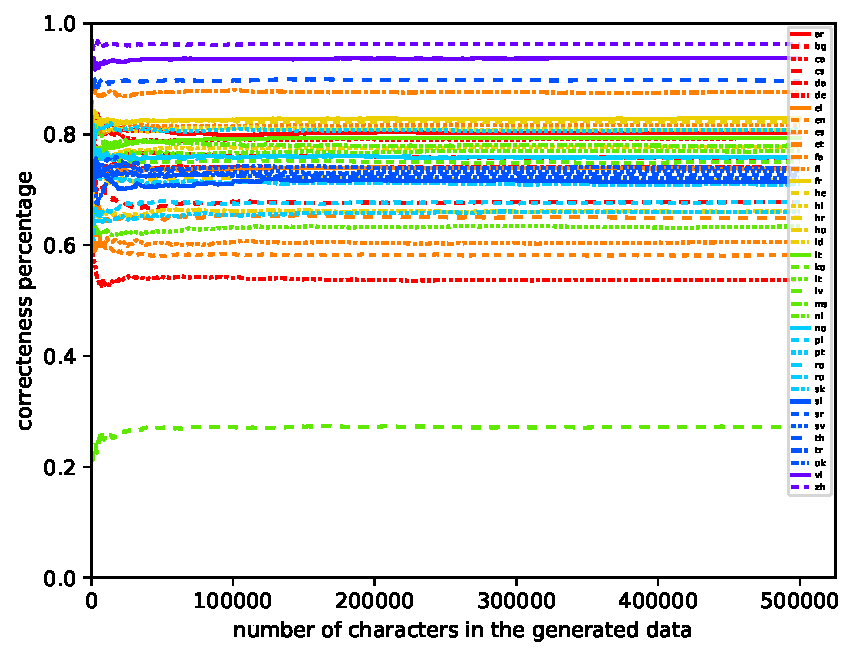
\includegraphics[width=0.7\textwidth]{graphs/lstm/gen_char_token_performance}
\caption{Correctness percentage of text generated by LSTM stabilizes by with increasing size.}
\label{Figure:lstm_gen_char_token_performance}
\end{figure}


\begin{figure}
\centering
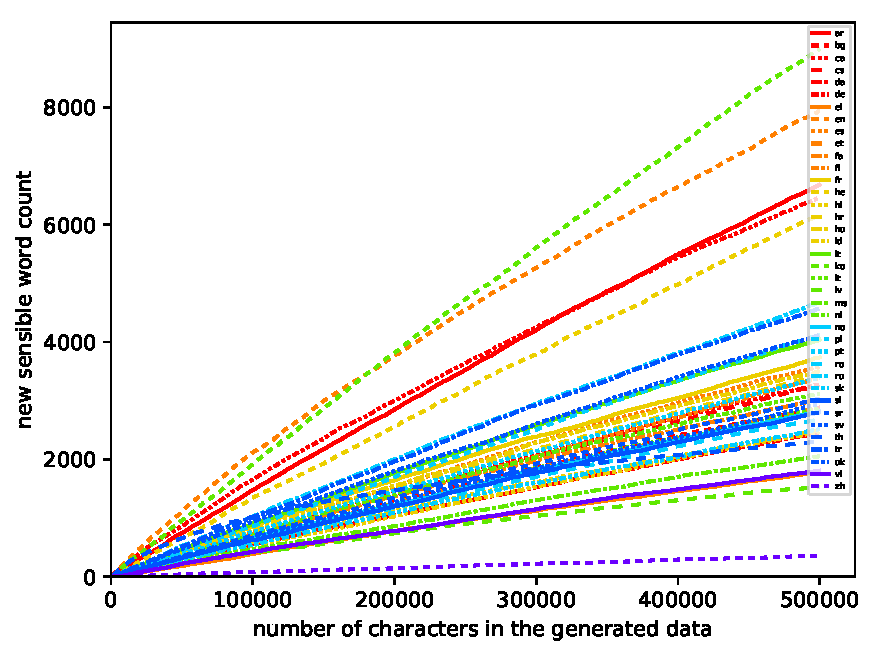
\includegraphics[width=0.7\textwidth]{graphs/lstm/gen_char_type_performance}
\caption{New sensible word count of text generated by LSTM increases steadily with increasing size.}
\label{Figure:lstm_gen_char_type_performance}
\end{figure}


For each language, and each of the four models, we then let the trained model generate 500,000 characters. We chose this because, the correctness percentage stabilises after approximately 250.000 characters, as can be seen in Figure \ref{Figure:lstm_gen_char_token_performance}. On the other hand, the number of new sensible words does not stabilise, as can be seen in Figure \ref{Figure:lstm_gen_char_type_performance}, but increases with the size of the generated data. For this reason, we sampled 500.000 characters for each language and model, for safety. 

The output was first tokenized by splitting by whitespace. As stated above in chapter \ref{section:methods}, we evaluated the percentage of words found in the generated data that were present in the reference corpora, and the number of words found in the generated data that were not present in the training data, but were present in the reference data. The results are presented below.

\begin{table}
\centering
\caption{Parameters used for all trained models}
\label{table:parameters}
\begin{tabular}{|l|l|}
        \hline
        RNN Size         & 128   \\
        Number of Layers & 2     \\ 
        Batch Size       & 50    \\ 
        Sequence Length  & 50    \\ 
        Number of Epochs & 50    \\ 
        Learning Rate    & 0.002 \\ 
        Decay Rate       & 0.97  \\
        \hline
    \end{tabular}
\end{table}


\chapter{Results} 

\section{Type Token Ratios}

\begin{figure}[h]
    \centering
    \begin{subfigure}[b]{0.32\textwidth}
    	\centering
        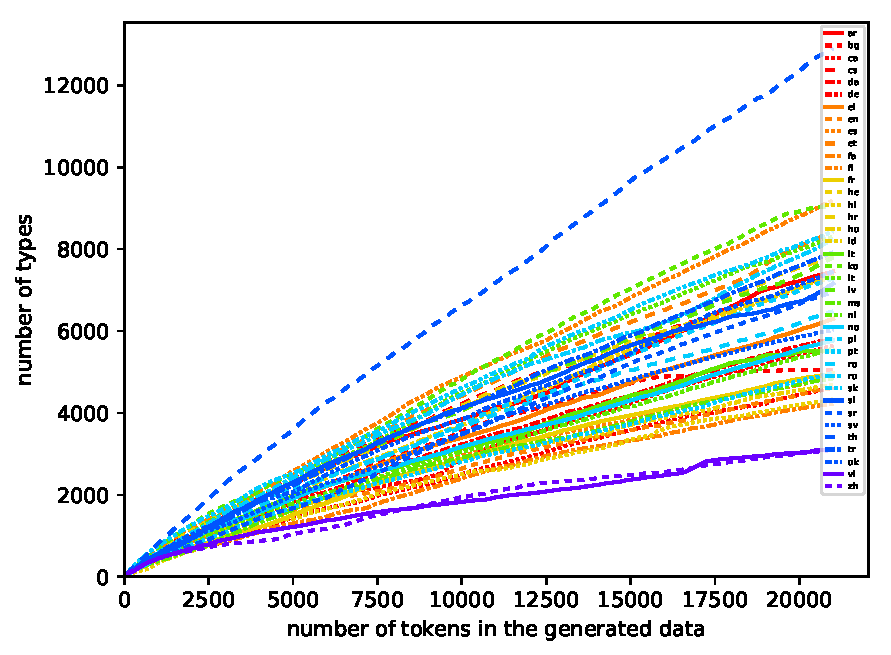
\includegraphics[width=\textwidth]{graphs/gensize_huge_types}
    \end{subfigure}
    \begin{subfigure}[b]{0.32\textwidth}
    	\centering
        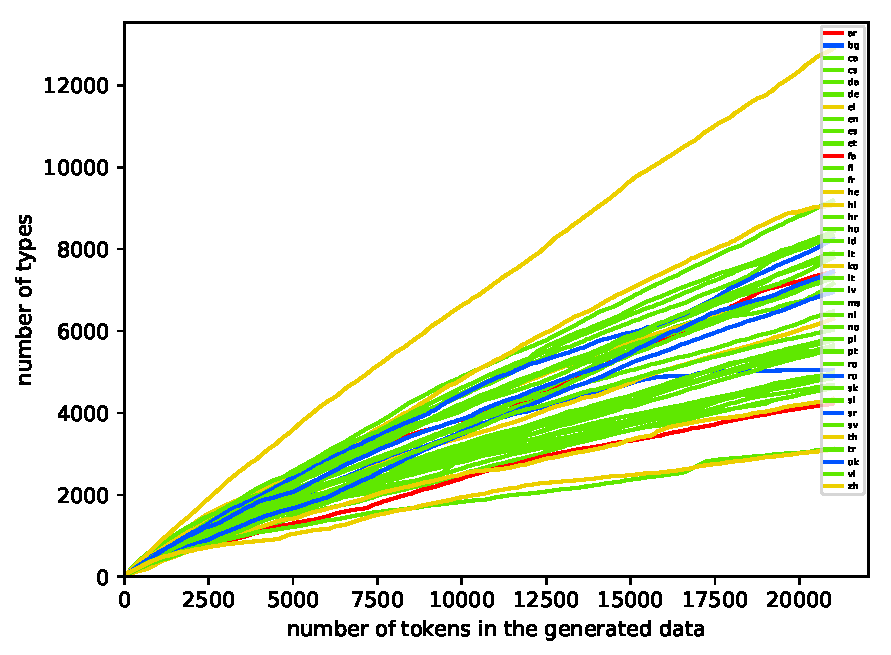
\includegraphics[width=\textwidth]{graphs/gensize_huge_types_script}
    \end{subfigure}
    \begin{subfigure}[b]{0.32\textwidth}
    	\centering
        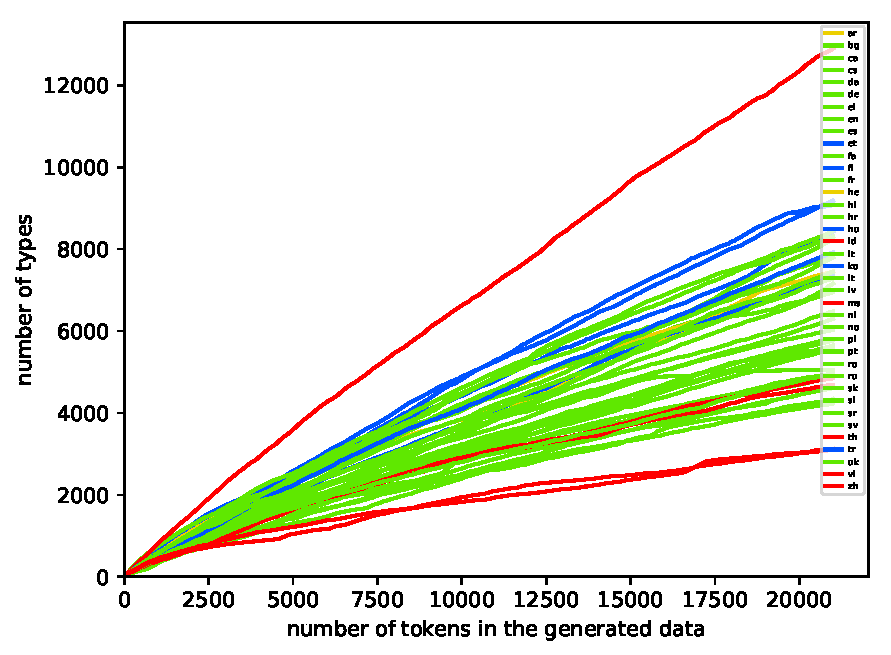
\includegraphics[width=\textwidth]{graphs/gensize_huge_types_morph_types}
    \end{subfigure}
    \caption{The type token ratios of the reference corpus, first colored individually, then by script (green is fusional, blue is agglutinative, red is isolating and yellow is introflexive) and by type (green is Latin, blue is Cyrillic, red is Arabic and yellow are others).}
    \label{Figure:gensize_huge_types}
\end{figure}

At first, we evaluate how good different models cover the type-token ratios for different languages. Figure \ref{Figure:gensize_huge_types} depicts the type-token ratios for the original data. They are fairly similar to each other, with the exception of Chinese and Vietnamese on the lower end, and Thai at the upper end. For Thai, this is because in Thai script, vowels are represented as diacritics above or below consonants, which means that there is a much larger number of characters than normal if a combination of a letter and a diacritic is counted as a character. This leads to a much higher number of different words than in other languages. (explanation needed for Vietnamese and Chinese). 
Interestingly, most languages type-token ratios rise consistently as the number of tokens is increased,while others, most notably Bulgarian, Arabic, and Russian, experience changes in slope. This could potentially be due to problems in the data, such as changes in topic or genre in the text. Interestingly, when looking at the data in terms of morphological typology, the agglutinative and the introflexive languages are close together in the upper region, while the isolating languages are generally at the bottom. The exception is Thai, which may be attributed to its script’s peculiarities. This is a result of how isolating languages have very few morphemes per word, resulting in a generally lower overall number of words, while agglutinative and introflexive languages have rather more different words than fusional languages, as fusional languages have the tendency to use one morpheme to denote multiple features. When looking at the same data in terms of scripts, there is a much less clear picture. The only interesting observation to be made here is that the languages using Cyrillic seem to have rather more unstable ratios in comparison to the languages using Latin or other scripts. 

When looking at the same graphs for the text generated by the LSTM, it is apparent that the ratios are similar to the ones in the original corpus. Generally, the ratios are slightly higher for each language. This will be explored further later for individual languages. The data is also more spread out, presumably because the ratios are now affected by the model’s different performance for the different languages. There are more outliers: Chinese, Vietnamese, Thai and Farsi towards the bottom and Latvian towards the top. This poses an interesting contrast to the ratios in the original data, because Thai was previously the language with the highest type/token ratio, it is now one of the lowest, presumably because the model didn’t succeed in generating the appropriate vowel diacritics. Farsi has also moved to a much lower position, which also indicates that the model didn’t work well. While there are no new interesting trends with regards to morphology types and scripts, it is interesting that there is much less fluctuation in the graphs of the generated data, further pointing to the fluctuations in the original data being due to topic changes or similar problems. The type/token ratios for the other three models are fairly similar; the difference for individual languages will be investigated in section  \ref{section:language_differences}.

\section{Results by Language}
\label{section:language_differences}

\subsection{Correctness Percentage Results}
The results for the correctness percentage evaluation are best described by grouping the languages by the performance of each of the four models investigated in comparison to each other. Using this idea, we form five groups: NAS GRU RNN LSTM; NAS GRU LSTM, RNN; NAS GRU LSTM RNN; NAS GRU RNN LSTM, and the group of results which are characterised not by the language order, but by the fact that these results are unusually close together. This group will be referred to as the ‘Close-Results Group.'

\subsubsection{Summary}
There are two main things to be learned from the analysis of correctness percentages across languages and models. The first is that type token ratios, in all our data, correlate with performance scores. The order of the models follows the rule that the better the correctness percentage, the closer the model’s ratio is to the type token ratio of the original data. This is promising, because for someone looking for a first indication of how well their model performed, the type token ratio is much easier to compute than the correctness percentage score. 

The second is that NAS and GRU almost universally have the best performance, while RNN is in most cases, but not in all, better than LSTM. This would indicate that NAS and GRU are best suited for the sort of machine learning that is required to produce correct words. This will be investigated further when looking at the number of new sensible words, as it will give an indication of how many of these correct words are remembered exactly from the training data, and how many have been newly generated by the model. 

The individual groups are discussed below.

\subsubsection{NAS $>$ $>$ GRU $>$ $>$ RNN $>$ $>$ LSTM}

\begin{figure}
\centering
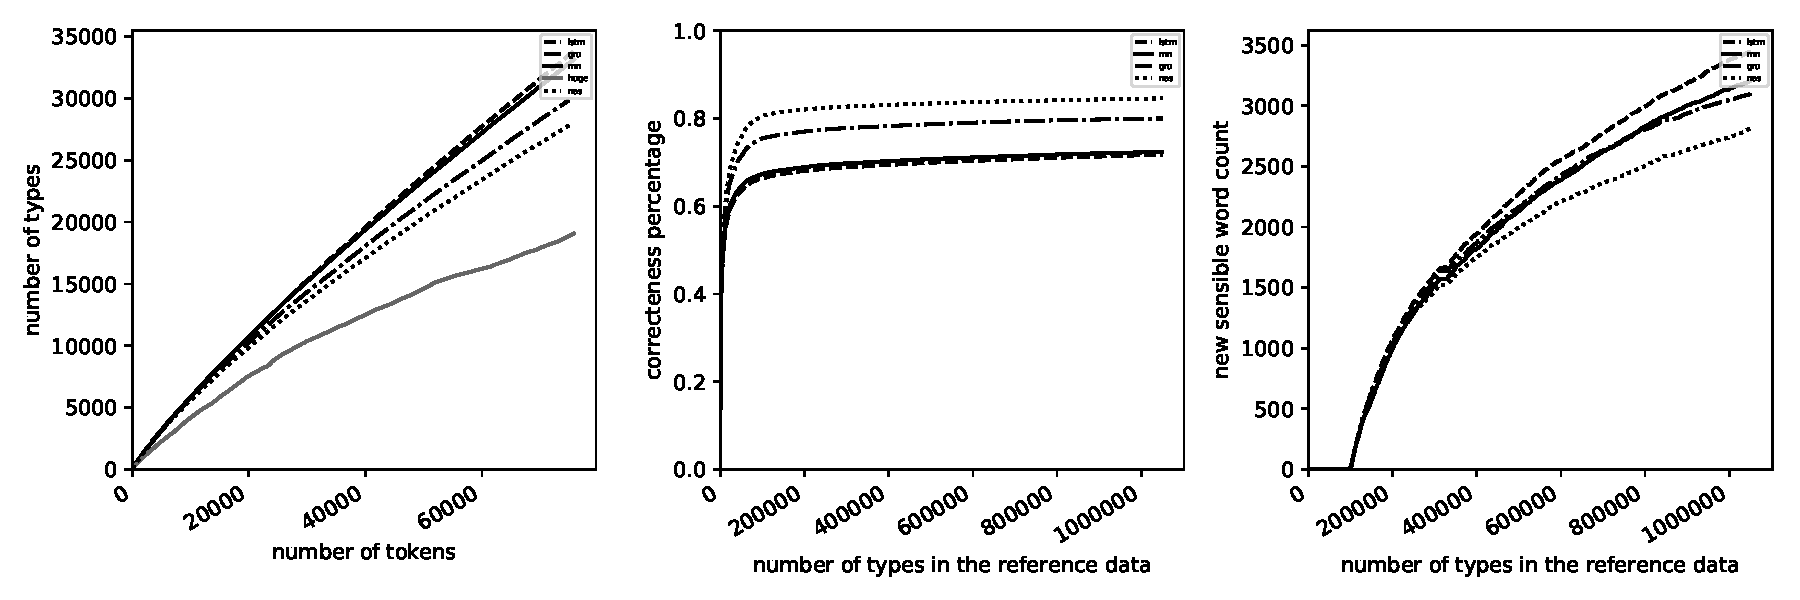
\includegraphics[width=\textwidth]{graphs/hr_all_graphs}
\caption{Performance scores for Croatian}
\label{Figure:hr_all_graphs}
\end{figure}

\begin{figure}
\centering
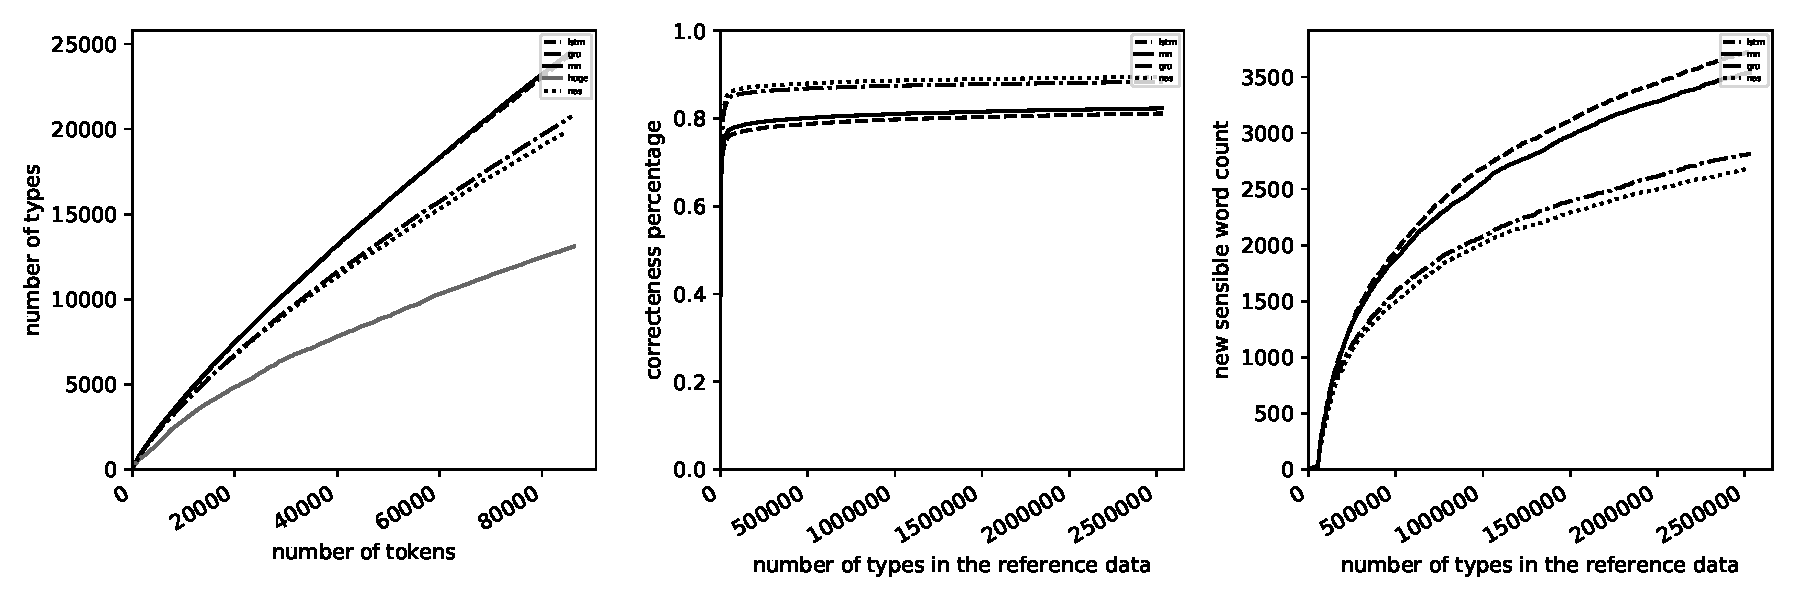
\includegraphics[width=\textwidth]{graphs/fr_all_graphs}
\caption{Performance scores for French}
\label{Figure:fr_all_graphs}
\end{figure}

In the first group, NAS has the best performance, followed by GRU, followed by RNN and then LSTM. The members of this group are Czech, Danish, Finnish, French, Croatian, Hungarian, Korean, Lithuanian, Polish, Portuguese, Romanian, Slovak, Serbian, Slovene and Ukrainian. 

Interestingly, the pattern for almost all of these languages is that RNN and LSTM form a group, as they are much closer to each other than they are to the other  group, NAS and GRU. Also, for most of these languages, RNN and LSTM are much closer together than NAS and GRU. The most extreme example of this is Croatian (Figure \ref{Figure:hr_all_graphs}), while in French (Figure \ref{Figure:fr_all_graphs}), the two groups are equally close together. Even though this shows that the phenomenon is not present in all languages to an equal degree, it is still significant, since it only occurs in this combination; NAS and GRU are never closer together than RNN and LSTM. This means that, when considering only the correctness percentage of the generated text, NAS has a greater advantage over GRU than RNN has over LSTM. 

Throughout all languages in this group, the order of the models for the type token ratios follows the order of the models for the correctness percentage, with the best performing model having the lowest type token ratio, thus the one which is closest to the ratio of the original data. This indicates that, for this group, the similarity of the type token ratios to the ones in the original data correlate with the correctness percentage, meaning that the fewer incorrect words were generated, the closer the generated model comes to a normal type token ratio. 

In terms of morphology types, this group consists mostly of fusional languages. Finnish and Hungarian are only exceptions, as they are both agglutinative (explanation?). Interestingly, no isolating or introflexive languages fall into this group. When looking at scripts, all languages in this group use Latin scripts, except for Serbian and Ukrainian, which use Cyrillic. It would make sense that there is no significant difference between languages using Latin and those using Cyrillic, as the two scripts have similar writing systems, concepts of vowels and consonants and word length, as opposed to scripts like Thai. This group, then, has the most members of any group, and also mostly has those with common attributes in our selection of languages: being fusional and using Latin or Cyrillic script. They are also mainly European languages.


\subsubsection{NAS $>$ GRU $>$ RNN $>$ LSTM}
\begin{figure}
\centering
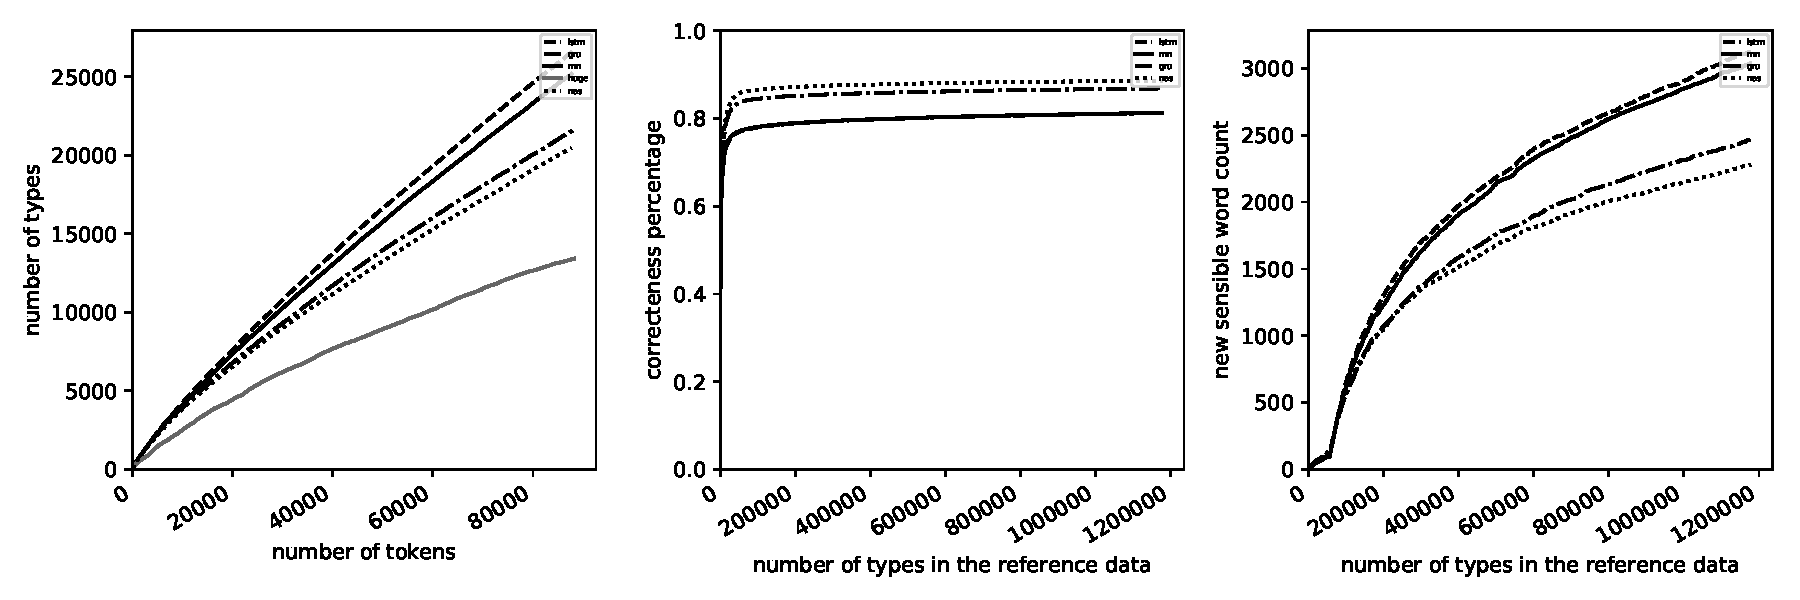
\includegraphics[width=\textwidth]{graphs/ca_all_graphs}
\caption{Performance scores for Catalan}
\label{Figure:ca_all_graphs}
\end{figure}
\begin{figure}
\centering
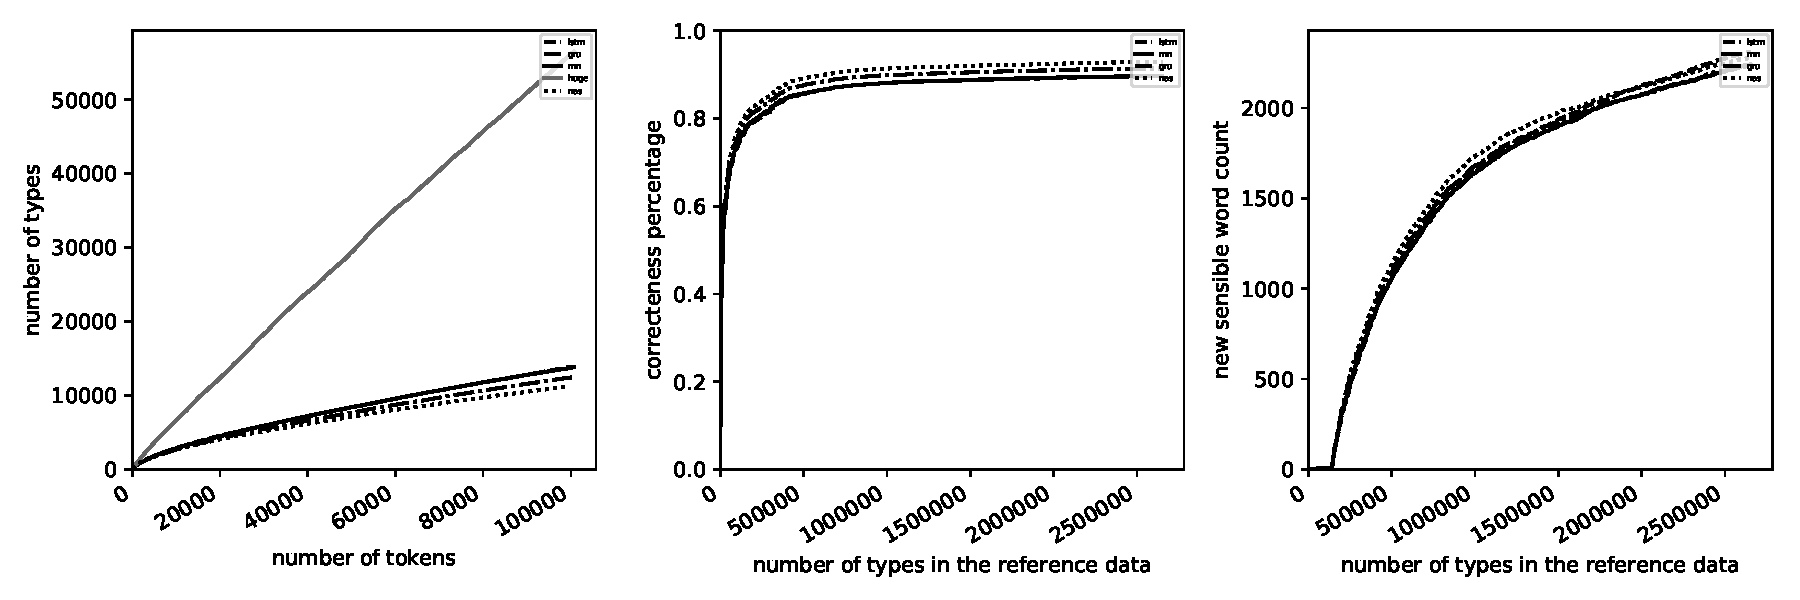
\includegraphics[width=\textwidth]{graphs/th_all_graphs}
\caption{Performance scores for Thai}
\label{Figure:th_all_graphs}
\end{figure}

The second group is similar to the first. NAS has the best performance, followed by GRU, followed by RNN and LSTM, which are so close together they are indistinguishable from one another in the graphs. The members of this group are Arabic, Bulgarian, Catalan, Greek, Farsi, Hindi, Indonesian, Malay, Dutch, Norwegian, Slovene, Thai and Turkish. 

The image is still largely similar to  the first group's, with the exception that RNN and LSTM are extremely close together. For most languages, NAS and GRU are much closer to one another than they are to the other two models, as can be seen in Figure \ref{Figure:ca_all_graphs}, for example. There is an exception to this, however, in Figure \ref{Figure:th_all_graphs}, where all the graphs are fairly close together. 

The type token ratios for this group are very interesting. While the pattern is similar to that of the first group, there is a difference visible between RNN and LSTM for most languages that are not visible with the correctness percentages. This is interesting because it suggests that differences that appear small with regards to the correctness percentage are magnified when looking at type token ratios, and also that it could be used as a further performance measure, as one would prefer to choose the model that more closely mirrors the properties of the original data, all other things being equal. 

Thai forms an exception in two ways. Firstly, the four models are rather closer together, with the distances between NAS, GRU, and the other two models being equally small. Secondly, and most remarkably, the type token ratios mirror the correctness percentages - similarly to the other languages in this group - but are much lower than the ratio in the original data, whereas it is the exact opposite for all other languages. This indicates that the models were unable to generate the diacritics used in the Thai script adequately,  resulting in a much lower number of different words overall. 

In contrast to the first group, most languages in this group are not European, with Dutch, Norwegian, Greek, Slovene, and Catalan as exceptions. Also in contrast to the first group, there are three isolating languages in this group, as well as one introflexive one. In terms of scripts used, about half of the languages use Latin. Interestingly, all the languages except for Dutch, Norwegian and Slovene have at least one of these features that makes them stand out, indicating that LSTM has the greatest advantage over RNN with fusional languages that use Latin. This is especially interesting because these are languages that are much more frequently used for analysis when comparing different language models, and using only these would indicate that LSTM is more significantly superior to RNN with regards to correctness percentages than it actually is.   

\subsubsection{NAS $>$ GRU $>$ LSTM $>$ RNN}
In the third group, NAS hast the best performance, followed by GRU, LSTM and finally RNN. NAS and GRU are in the same order as in the first two groups, but LSTM performs better than RNN. The languages in this group are Spanish, Estonian, Hebrew, Italian, and Russian. 

Similarly to the first group, the distance between GRU and LSTM is much greater than the one between NAS and GRU, and LSTM and RNN respectively. The performance gap between RNN and LSTM is as big as the one between NAS and GRU, or smaller. The type-token ratios, as for the first group, are indicative of performance.

Half of the languages in this group are fusional, while Estonian is an agglutinative and Hebrew introflexive. Almost all languages in this group use Latin script, with Russian, which uses Cyrillic, being the exception. In this regard, little distinguishes this group from the first group, in which RNN had better performance than LSTM. 

\subsubsection{Close-Results Group}
The fourth group consists of languages where the performances of the four models are very close together, in various orders. This group consists of Korean, Vietnamese, and Chinese. 

The actual orders, although they are hard to distinguish, are GRU LSTM RNN NAS for Korean, NAS GRU LSTM RNN for Chinese, and NAS GRU RNN LSTM for Chinese. Though these are different, the group is held together by the fact that the performances of the models differ only very slightly when compared to most other languages. 

When looking at type token ratios, these are all languages that show a much lower type token ratio in the original data than in all the different generated data. Also, as was the case in the group in which RNN and LSTM where indistinguishable from one another, there are far greater differences to be observed in the type token ratios than in the correctness percentages. 

This group is also extraordinary because Chinese and Vietnamese are isolating languages while Korean is an agglutinative language. This is an extreme contrast to the other groups, which consist of predominantly fusional languages. Similarly, neither Chinese nor Korean use Latin script, also in contrast to most of the other languages investigated. 

\subsubsection{NAS $>$ GRU $>$ RNN $\gg$ LSTM}
In the fifth group, LSTM has a significantly worse performance than the other three models. The group includes German, English, and Latvian. The order of the models is the same as in the first group: NAS GRU RNN LSTM, but there is a significant difference: the distance between RNN and LSTM is several times greater than any of the distances between the other models. As in the first group, the differences in correctness percentage are perfectly mirrored in the type token ratios. 

There is no apparent explanation why these three languages in particular exhibit this pattern. German, English, and Latvian are all fusional European languages that use Latin script. German is a language with a relatively large amount of morphology while English has very little, within the boundaries of fusional languages. English and German are the languages with the most data in the Wikipedia corpus, while Latvian has comparatively little data. The only criterion that they apparently share is that an LSTM aseems to have significant difficulty outputting correct words in them. 

\subsection{New sensible word count results}
The results for the new sensible word count evaluation can also be described by grouping the languages by the relative performance of the four models, although they form a larger number of groups and therefore a less clear picture than for the correctness percentages. We observe five groups, in addition to six single languages that could not be assigned a group. These are: LSTM RNN GRU NAS; LSTM RNN NAS, GRU; LSTM RNN NAS GRU; LSTM space RNN NAS, GRU, and LSTM NAS RNN GRU. Latvian, Chinese, Greek, Spanish, Thai, and Vietnamese all form single language groups. 

\subsubsection{Summary}
In contrast to the results for the correctness percentages, there is a less clear picture to be seen when considering all groups for the new sensible word count results. This is largely due to six individual languages having no pattern in common with any other language. Apart from that, the pattern is similar: three groups that differ only in the order of the last two models, one other group, and one group where LSTM has a large performance difference to all other models. 

One thing that we can learn from these groups is that, unlike the correctness percentages, they are not directly mirrored in the type token ratios. While it sometimes seems that that is the case, this is because for some groups, the order of the models is similar to the order from the correctness percentages in reverse. However, there is no correlation from the type token ratios to the number of new sensible words. Another conclusion that can be drawn is that in general, LSTM performs better than RNN, which performs better than the other languages. This is the reverse picture of the one for the correctness percentages. This indicates that the more a model is able to generate correct words, the less it is able to capture character-level dependencies and generated new sensible words that did not occur in the training data. 

\subsubsection{LSTM $>$ RNN $>$ GRU $>$ NAS}

\begin{figure}
\centering
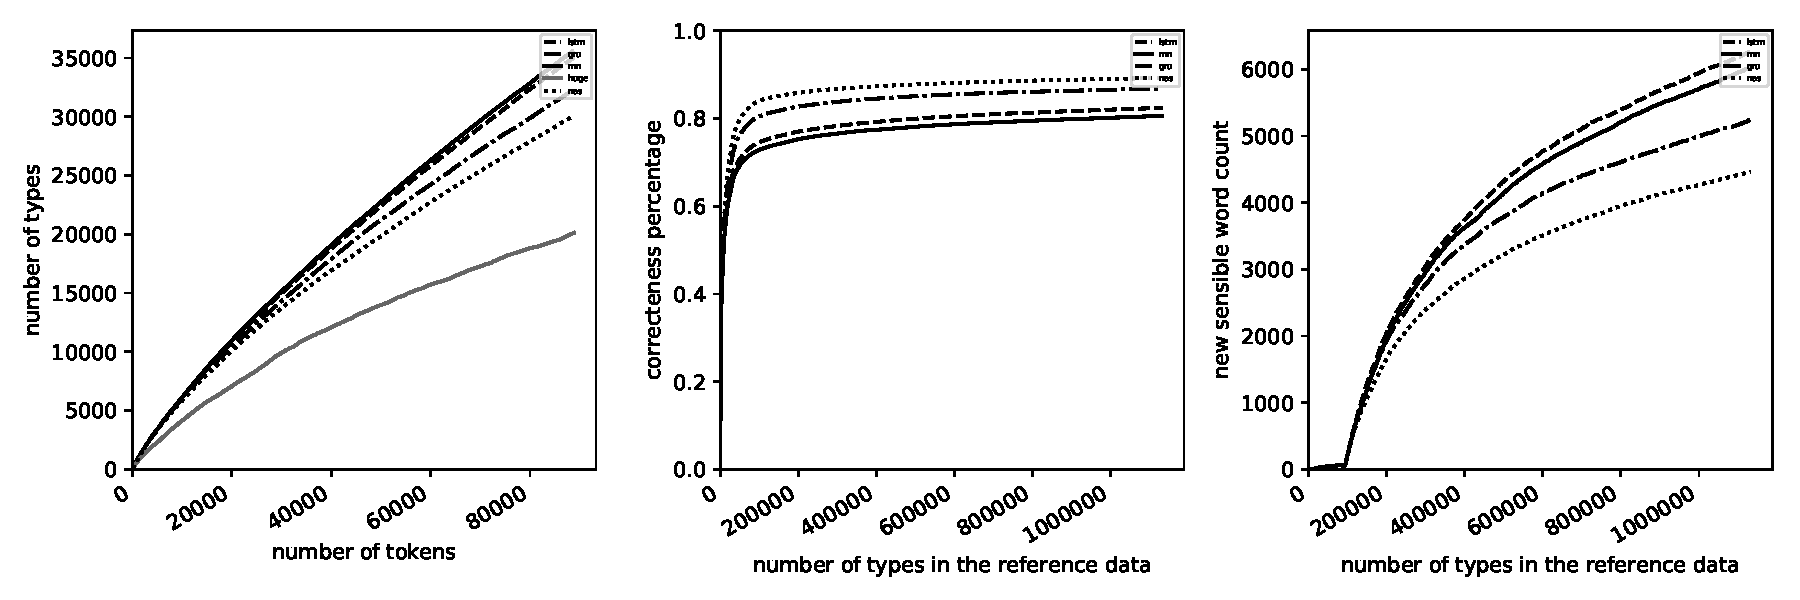
\includegraphics[width=\textwidth]{graphs/he_all_graphs}
\caption{Performance scores for Hebrew}
\label{Figure:he_all_graphs}
\end{figure}

\begin{figure}
\centering
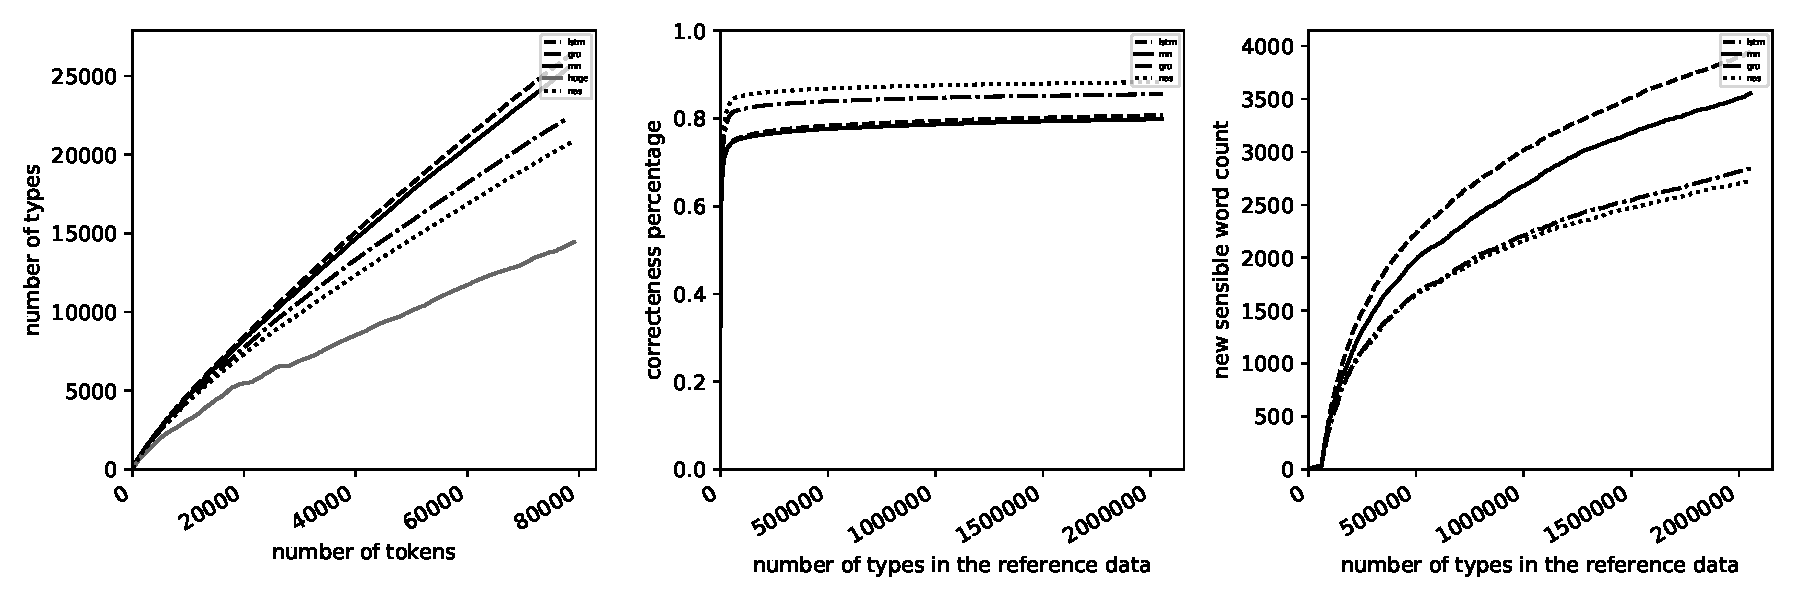
\includegraphics[width=\textwidth]{graphs/it_all_graphs}
\caption{Performance scores for Italian}
\label{Figure:it_all_graphs}
\end{figure}

\begin{figure}
\centering
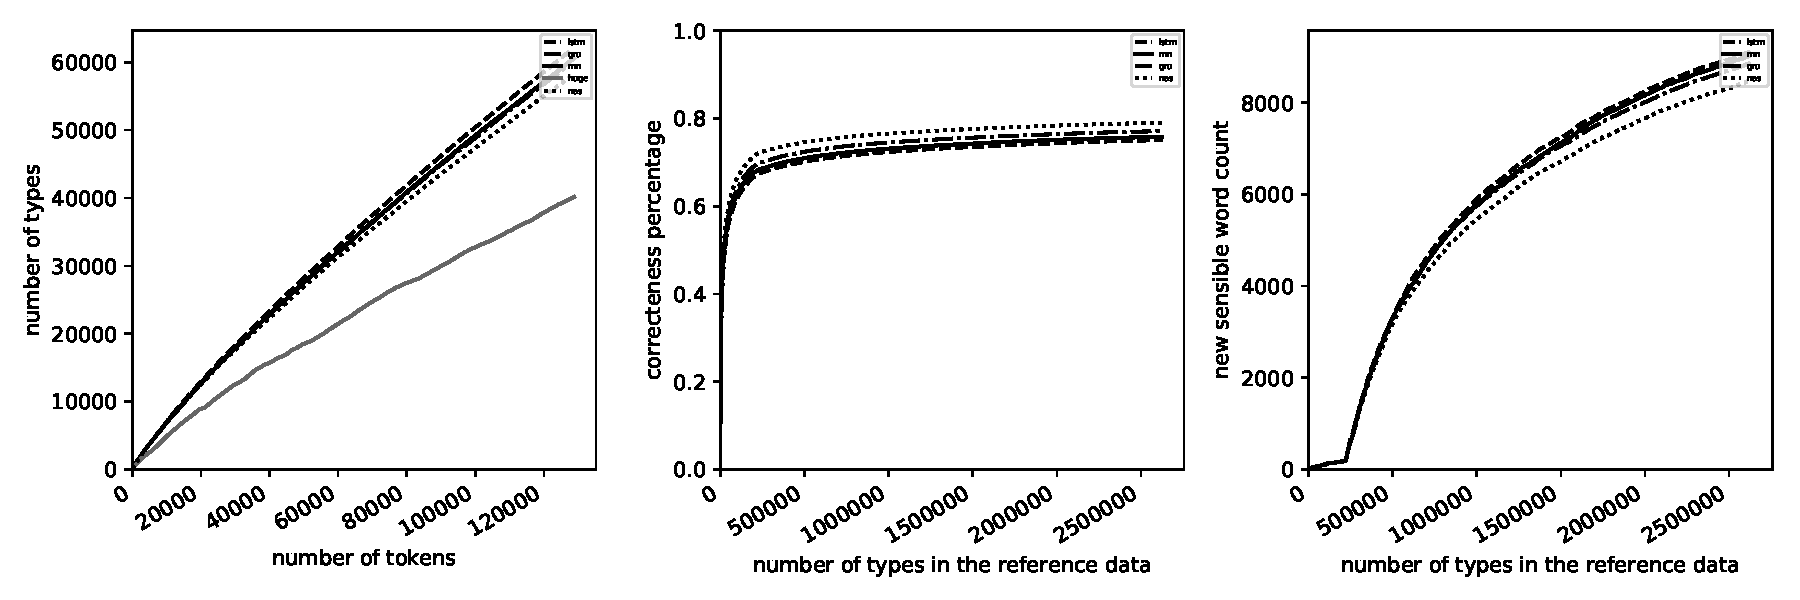
\includegraphics[width=\textwidth]{graphs/ko_all_graphs}
\caption{Performance scores for Korean}
\label{Figure:ko_all_graphs}
\end{figure}

\begin{figure}
\centering
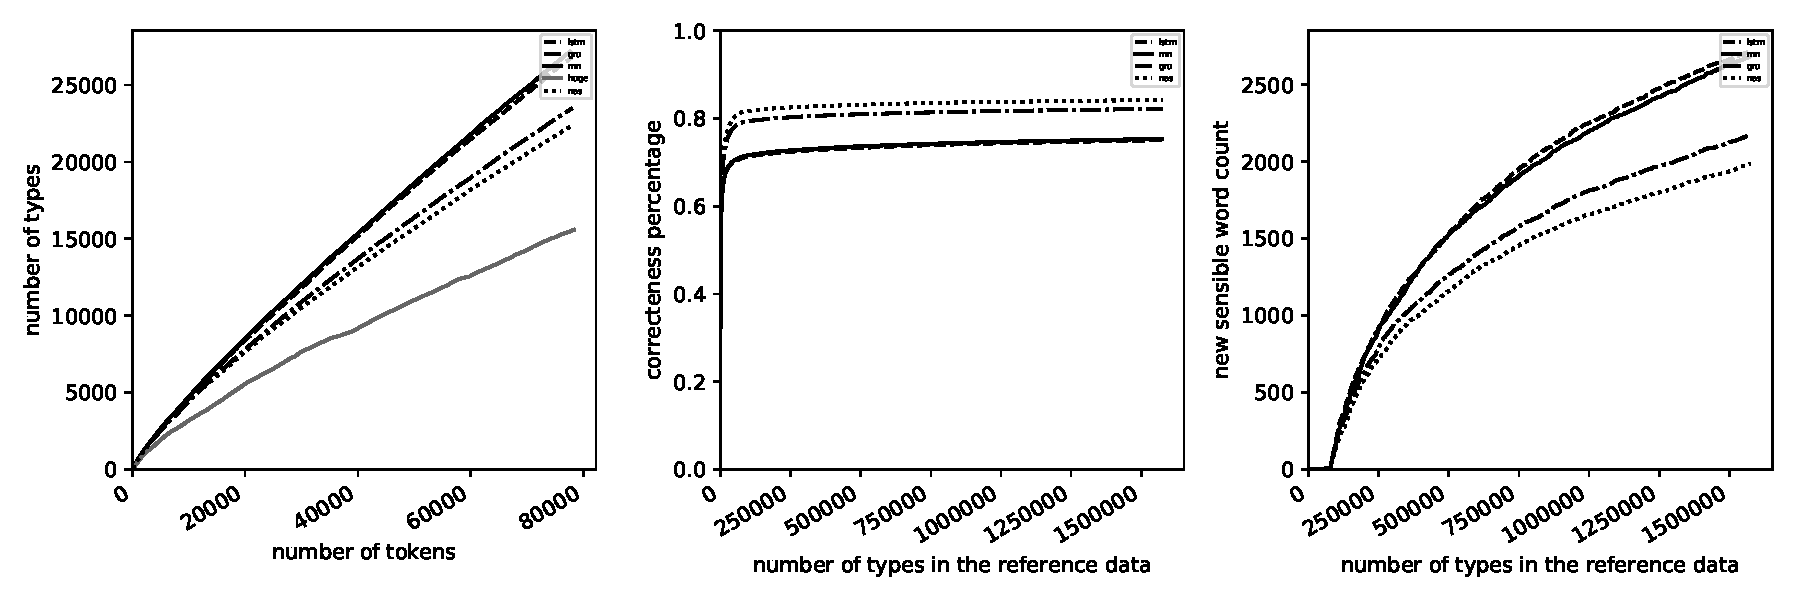
\includegraphics[width=\textwidth]{graphs/no_all_graphs}
\caption{Performance scores for Norwegian}
\label{Figure:no_all_graphs}
\end{figure}

In first and the largest group,  LSTM has the best performance, followed by RNN, GRU, and NAS. The group includes Catalan, Danish, Farsi, French, Hebrew, Hindi, Croatian, Italian, Korean, Norwegian, Romanian, Russian, and Turkish. 

The pattern for these languages is that LSTM and RNN have the best performance, followed by GRU and NAS. As in the first group of correctness percentages, LSTM and RNN, and GRU and NAS are closer together than they are to the other group. A typical example of this is Norwegian (Figure \ref{Figure:no_all_graphs}). There are some cases where this is less pronounced, such as Italian (Figure \ref{Figure:it_all_graphs}) or Hebrew (Figure \ref{Figure:he_all_graphs}), but in general there seems to be less of a difference between LSTM and RNN, and GRU and NAS, than between RNN and GRU. 

Two languages belonging to this group exhibit slightly different patterns: Korean (Figure \ref{Figure:ko_all_graphs}) and Croatian (Figure \ref{Figure:hr_all_graphs}). The order of the models is the same, but for Korean the models are extremely close together compared to the other languages in this group. This is to be expected, as Korean was in the 'close results' group  for token performance. Croatian is the other exception, as RNN and GRU are so close together in this group that they cross each other several times. The graphs are also more irregular than usual, pointing to possible problems in the data. 

Most of the languages in this group are fusional and use Latin script. The exceptions are Korean and Turkish, which are agglutinative, and Hebrew, which is isolating. Farsi, Hindi, Korean, and Russian all use scripts other than Latin. It is also interesting that only half of the languages in this group are European languages.

\subsubsection{LSTM $>$ RNN $>$ NAS,GRU}
\begin{figure}
\centering
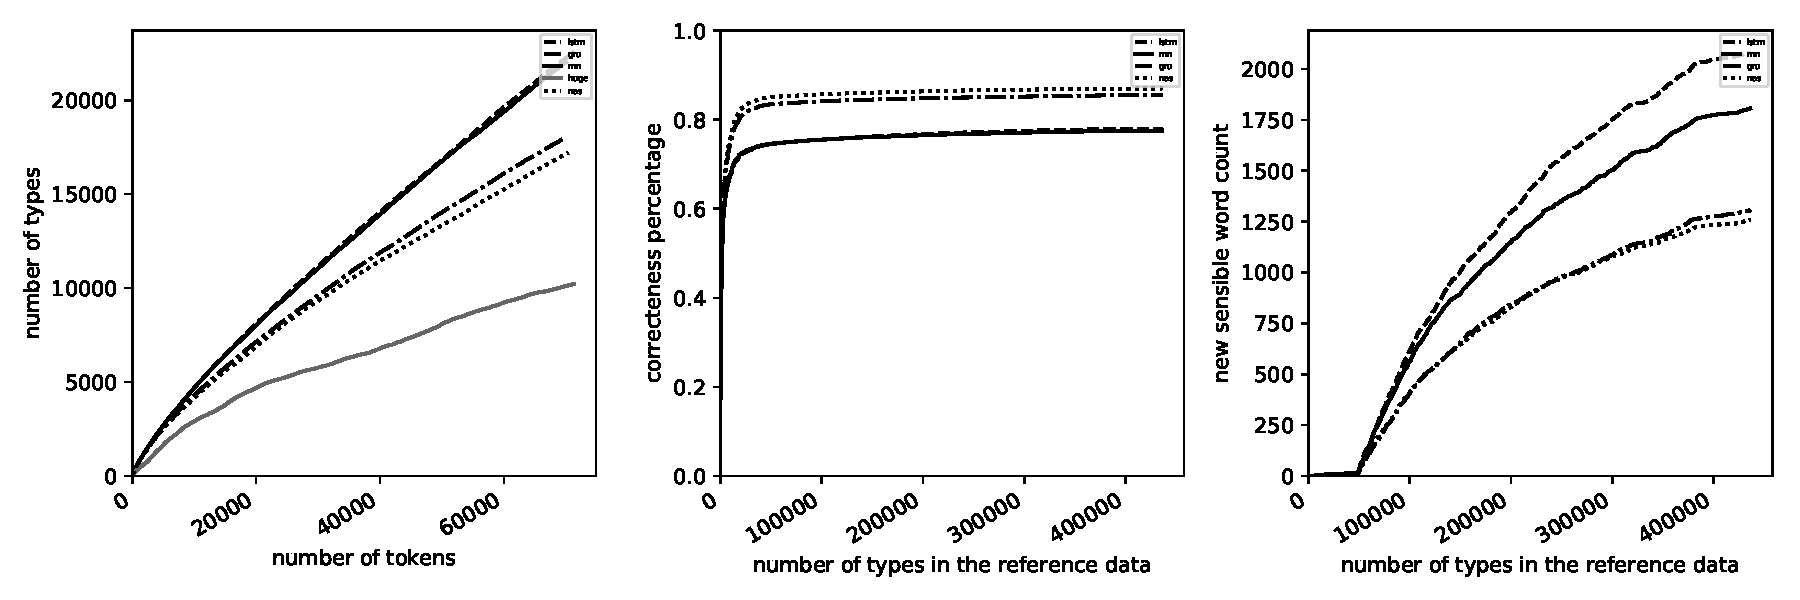
\includegraphics[width=\textwidth]{graphs/ms_all_graphs}
\caption{Performance scores for Malay}
\label{Figure:ms_all_graphs}
\end{figure}

\begin{figure}
\centering
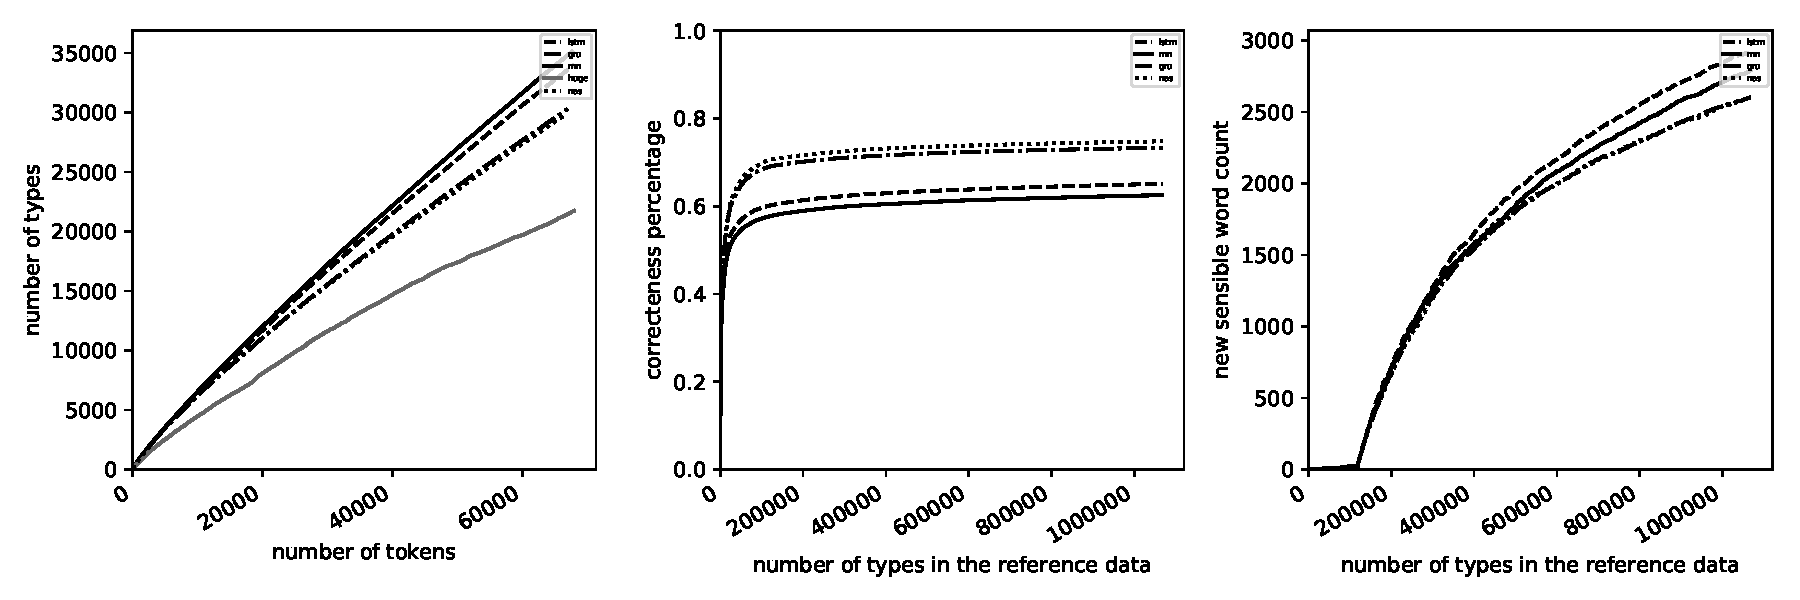
\includegraphics[width=\textwidth]{graphs/et_all_graphs}
\caption{Performance scores for Estonian}
\label{Figure:et_all_graphs}
\end{figure}

In the second, much smaller, group, LSTM has the best performance, followed by RNN, then NAS, with GRU very close behind. The members of this group are Bulgarian, Estonian, Malay, Portuguese and Serbian. There are some differences within the group with regards to the difference in performances between models, ranging from Malay (Figure \ref{Figure:ms_all_graphs}), where the differences are comparatively large, to Estonian (Figure \ref{Figure:et_all_graphs}), where they are comparatively small. 

Interestingly, over half of the languages in this group are eastern European languages. All except Malay are fusional, and all but Bulgarian and Serbian use Latin. This makes it a relatively mixed group with no clear feature to bind it together, except possibly that none of the languages use a script other than Latin or Cyrillic, which are relatively similar. 

\subsubsection{LSTM $>$ RNN $>$ NAS $>$ GRU}

\begin{figure}
\centering
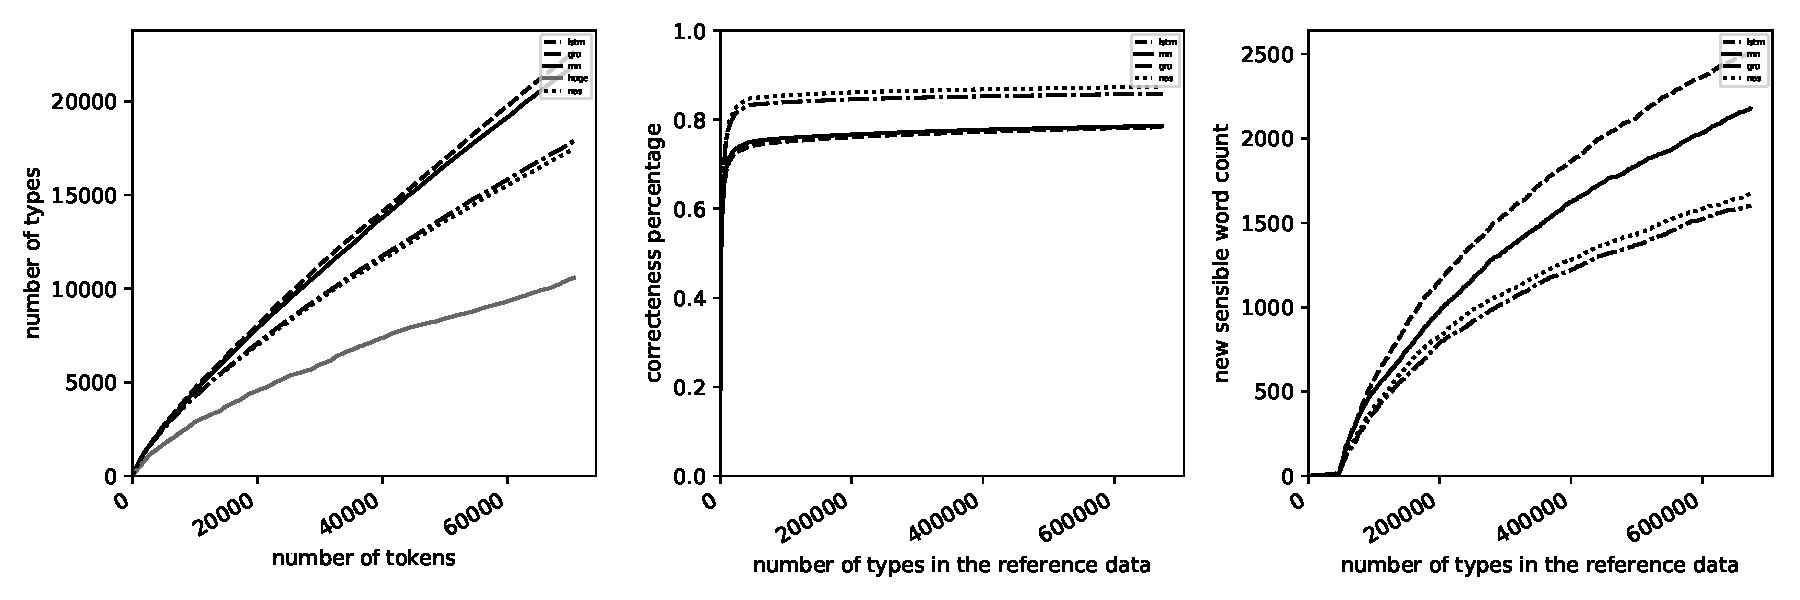
\includegraphics[width=\textwidth]{graphs/id_all_graphs}
\caption{Performance scores for Indonesian}
\label{Figure:id_all_graphs}
\end{figure}

\begin{figure}
\centering
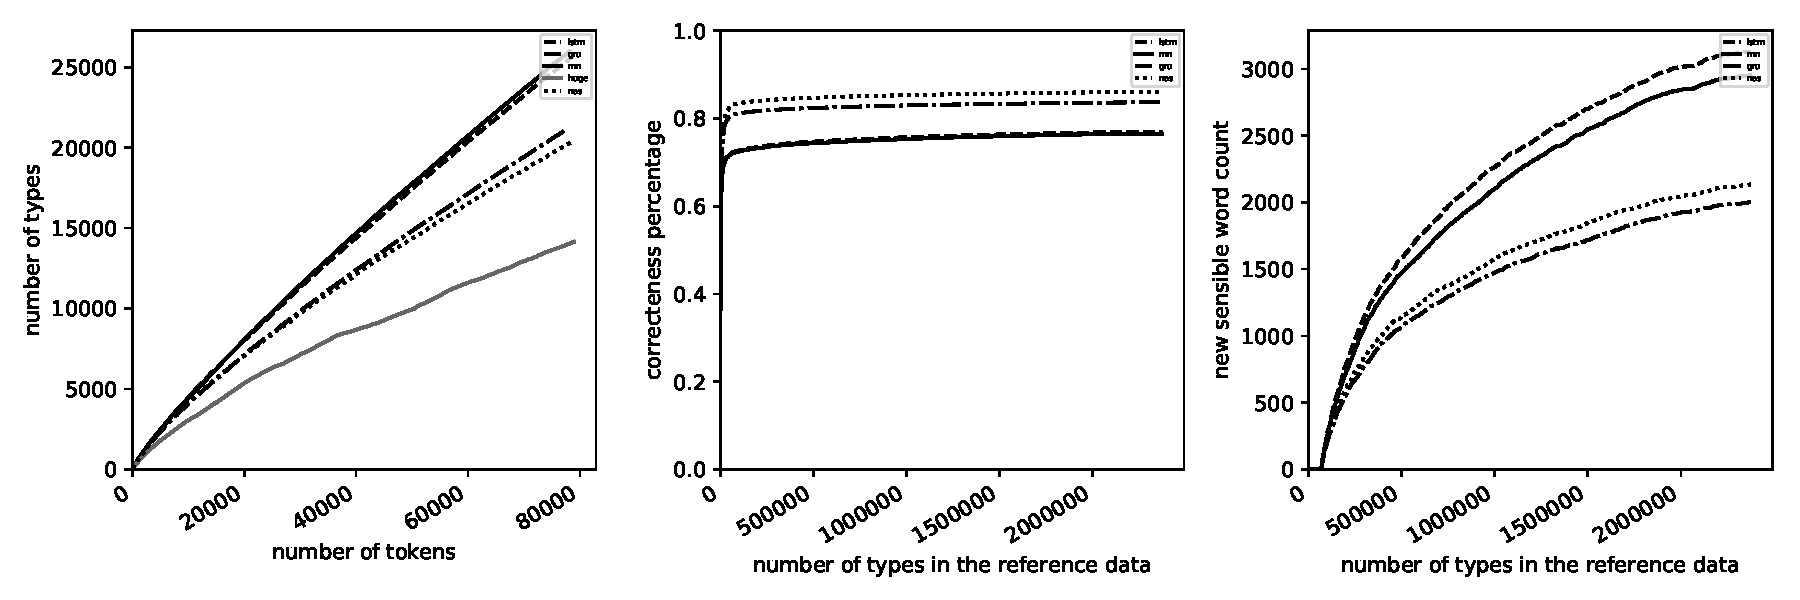
\includegraphics[width=\textwidth]{graphs/nl_all_graphs}
\caption{Performance scores for Dutch}
\label{Figure:nl_all_graphs}
\end{figure}

\begin{figure}
\centering
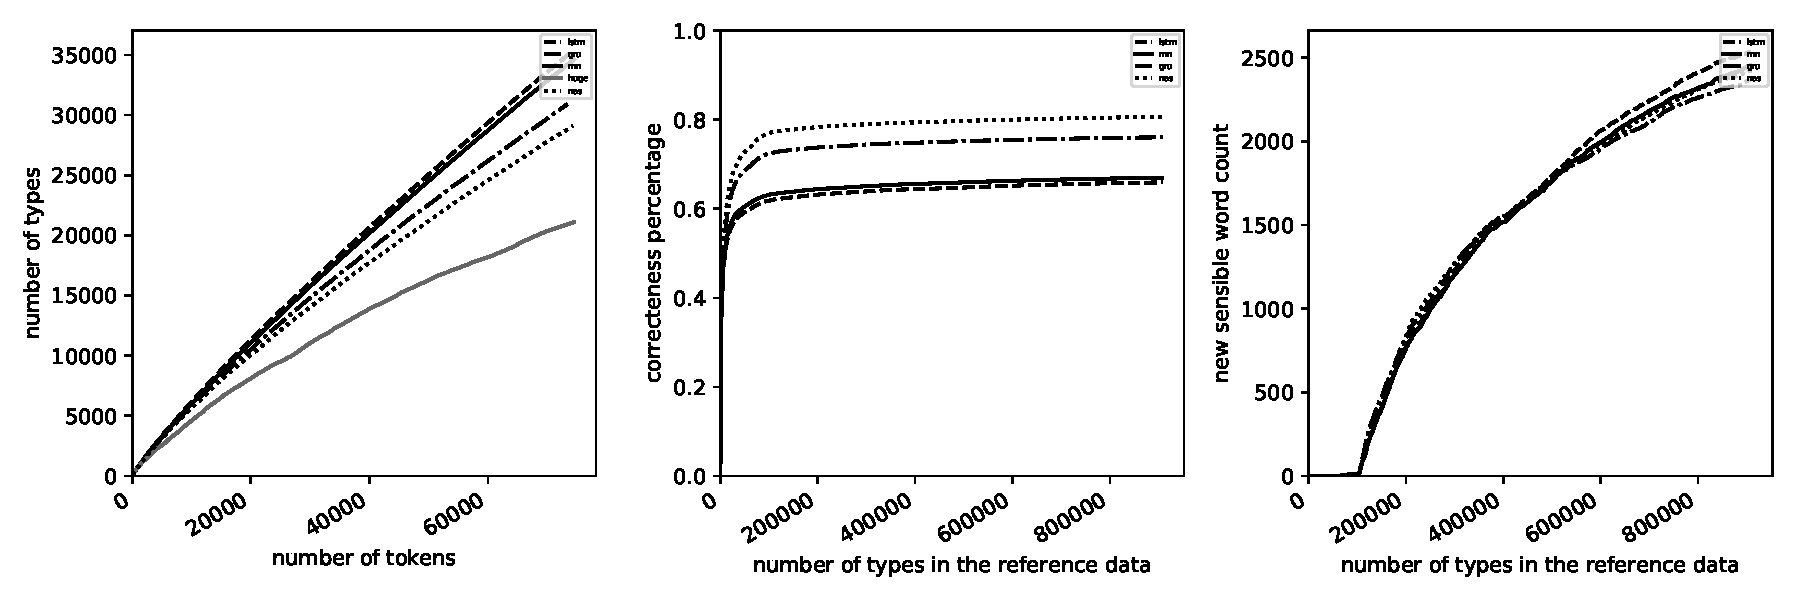
\includegraphics[width=\textwidth]{graphs/sk_all_graphs}
\caption{Performance scores for Slovak}
\label{Figure:sk_all_graphs}
\end{figure}

In the third group, LSTM performed best, followed by RNN, NAS and then GRU. This group consists of Arabic, Czech, Indonesian, Dutch, Slovak, Slovene, Swedish, and Ukrainian. The patterns are very similar to the first group, except for NAS being better than GRU. As with the first group, LSTM and RNN, as well as NAS and GRU, are closer together than they are to the other group. If one of the groups has more space in between than the other, it is always LSTM and RNN, as can be seen in Figure \ref{Figure:id_all_graphs}. If not, the groups are frequently equally close together, as in Figure \ref{Figure:nl_all_graphs}. Slovak is an exception, as RNN and NAS are extremely close together for this language (Figure \ref{Figure:sk_all_graphs}), although they are still distinguishable from one another. 

In terms of morphology types and scripts, this group is even more heterogenous than the first group, including Arabic, an introflexive language which uses the Arabic script, Indonesian, which is an isolating language, and Ukrainian, which uses Cyrillic. There also seems to be no significant difference to the languages in the first group, where GRU performs better than NAS. 

\subsubsection{LSTM $>$ NAS $>$ RNN $>$ GRU}
In the fourth group, LSTM has the best performance, followed by NAS,  RNN and then GRU. This group includes Finnish, Hungarian, Lithuanian, and Polish. The patterns in this group are very interesting, because in three out of four languages, the graphs of the models cross each other fairly late, or even several times, meaning that which model performs best is highly dependent on how much reference data is considered. This is unusual and suggests that there are advantages for some models that only pay off if enough reference data is available. The mix of languages is also interesting: while half of them are agglutinative and half are fusional, they are all Eastern European, which raises interesting questions as to what binds them together. 

\subsubsection{LSTM $\gg$ RNN $>$ GRU $>$ NAS}
In the fifth group, LSTM has the best performance by far, followed by RNN, GRU and NAS. This group consists of English and German and is one of the more unusual groups. It obviously mirrors the group for correctness percentages which consists of English, German, and Latvian, and in which the order of the models is the exact reverse of those in this group, including the large gap between LSTM and RNN. However, Latvian is missing from this group. 

There is still no clear indication of why English and German show such unique performance patterns. Both languages are fusional and use Latin script. Their only feature that stands out is that they are the languages for which the most data is available in the Wikipedia corpus. It might be possible that the size of the data somehow correlates with the quality of the data or with how diverse the vocabulary used is, which then leads to LSTM achieving much better performance. 

\subsubsection{Unique pattern group}
The sixth group includes all languages that could not be assigned a group, as they have a unique pattern that they do not share with any other language. The group consists of Greek, Spanish, Latvian, Thai, Vietnamese, and Chinese. The patterns of each of these languages do not stand out particularly on their own, but it is noteworthy for each of them that they are the only languages with that pattern, meaning that there must be something that distinguishes them from all other languages. 

Most of the languages in this group have some trait that may be responsible for their different behaviour. Chinese, Thai, and Vietnamese are all isolating languages, which also means that the majority of isolating languages fall into this category, suggesting that some property of isolating languages makes them more likely to have unusual new sensible word count performance. Estonian is also notable for being an agglutinative language. Also, three of the six languages in this group use a script other than Latin or Cyrillic. This suggests that these scripts are more likely to lead to unusual performance patterns. 

\subsection{Recommendations}
Using both these performance metrics, there are some recommendations that we can give regarding the choice of models. These recommendations are based on the information gained from the analysis of both the correctness percentages and the new sensible word counts. While it is common for most languages and models that there is a direct trade-off, meaning that the better a model performs with regard to correctness percentage, the worse it performs with regard to the new sensible word count, and vice versa, there are some cases in which one model is superior to at least one other model in both cases. This means that the model which is always inferior can be eliminated from the list of models that are considered for the task. We present a list of such recommendations together with the languages to which they apply. The general picture is that we are unable to give recommendations for some languages, but for most languages  NAS is always better than GRU, or LSTM always better than RNN, or both. There are several exceptions where we can even give a definite order. 

The first group is that for which NAS always performs better than GRU, with a trade-off between NAS, RNN, and LSTM. The result of this is that there is no reason to use GRU. The group includes Portuguese, Serbian, Czech, Slovak, and Swedish. The pattern for these languages is that the order for correctness percentages is NAS GRU RNN LSTM while the order for the new sensible word count is LSTM $>$ RNN $>$ NAS $>$ GRU, or LSTM $>$ RNN with NAS and GRU extremely close together. 

The second group is that for which LSTM always performs better than RNN, with a trade-off between LSTM, GRU, and NAS. This means that there is no reason to use RNN for any of the languages between this group. The group includes Catalan, Farsi, Hebrew, Hindi, Italian, Norwegian, Turkish, and Russian. The pattern for this group is NAS $>$ GRU $>$ RNN $>$ LSTM or NAS $>$ GRU with RNN and LSTM very close together for the correctness percentage and LSTM $>$ RNN $>$ GRU $>$ NAS.  

The third group is that for which LSTM is better than RNN and NAS is better than GRU, with a remaining trade-off between LSTM and NAS. This means that depending on the application, it is most sensible to choose only between LSTM and NAS. This group includes Arabic, Bulgarian, Greek, Indonesian, Malay, Dutch, Slovene, and Thai. The pattern of this group is that the order is NAS $>$ GRU $>$ LSTM $>$ RNN (or LSTM and RNN close together) for the correctness percentage, and LSTM $>$ RNN $>$ NAS $>$ GRU (or NAS and GRU close together) for the new sensible word count, except for Thai, which has a unique pattern. 

The fourth group is that in which NAS is better than both RNN and GRU, resulting in a trade-off only between NAS and LSTM. This group consists of Finnish, Hungarian, Latvian, and Polish. The pattern for these languages is that the correctness percentage order is NAS $>$ GRU $>$ RNN $>$ LSTM and the order for the new sensible word count is LSTM $>$ NAS $>$ RNN $>$ GRU. 

Furthermore, there are several languages in which there is a unique order of preference for the models. These are shown in table \ref{table:laguage-wise-reccommendations}.

Finally, we can give no recommendation for Danish, German, English, Spanish, French, Croatian, Korean, and Romanian. With the exception of Spanish, all languages in this group have the order NAS GRU RNN LSTM for correctness percentage, and the reverse order for the new sensible word counts. The choice of models for this group depends entirely on the priorities of the user, which is particularly unfortunate as the group includes some of the world’s most frequently used languages.

\begin{table}[]
\centering
\caption{Recommended models per language for either best token or type performance, from best to worst.}
\label{table:laguage-wise-reccommendations}
\def\arraystretch{1.5}%  1 is the default, change whatever you need
\begin{tabularx}{\textwidth}{XllX}
\textbf{Language}              & \textbf{Token}   & \textbf{Type}    & \textbf{Don't use} \\ \hline \hline
DA, DE, FR, HR, KO, RO, EN, ES & NAS $>$ GRU $>$ RNN $>$ LSTM & LSTM $>$ RNN $>$ GRU $>$ NAS &                    \\ \hline
PT, SR, CS, SK, SV             & NAS $>$ RNN $>$ LSTM     & LSTM $>$ RNN $>$ NAS     & GRU                \\ \hline
CA, FA, HE, HI, IT, NO, TR, RU & NAS $>$ GRU $>$ LSTM     & LSTM $>$ GRU $>$ NAS     & RNN                \\ \hline
AR, BG, ET, ID, MS, NL, SL, TH & NAS $>$ LSTM         & LSTM $>$ NAS         & RNN, GRU           \\ \hline
FI, HU, LT, PL                 & LSTM $>$ NAS         & NAS $>$ LSTM         & RNN, GRU           \\ \hline
LV                             & NAS              & NAS              & RNN, LSTM, GRU     \\ \hline
ZH                             & RNN              & RNN              & LSTM, GRU, NAS     \\ \hline
EL                             & NAS $>$ GRU $>$ LSTM     & LSTM $>$ NAS $>$ GRU     & RNN                \\ \hline
VI                             & LSTM             & LSTM             & RNN GRU NAS       
\end{tabularx}
\end{table}

\section{Results by Model}
\subsection{Correctness Percentage}
The correctness percentage increases with the size of the reference data, in accordance with Heap’s Law. This means that it will always increase, although only slightly, meaning that there is no good point at which one can decide that this is the definite correctness percentage. For this reason, we compute the correctness percentage using reference data which, for each language, has been shortened to the length of the smallest reference data - namely, Chinese - in order to compute the languages fairly.
There are several general conclusions to be drawn from this investigation of correctness percentages for all four models. Firstly, as we had already concluded from our discussion of correctness percentages for all languages, LSTM and RNN perform worse in general than NAS and GRU. Secondly, in most cases, agglutinative languages perform rather better and isolating languages rather worse than average. The differences between the models are discussed below. 
\subsubsection{NAS}

\begin{figure}[h]
    \centering
    \begin{subfigure}[b]{0.32\textwidth}
    	\centering
        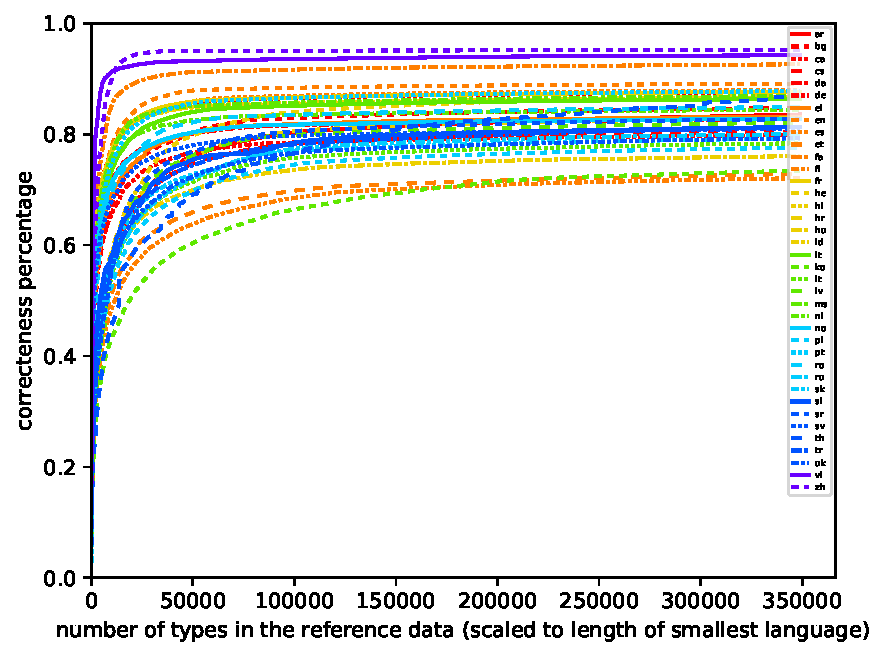
\includegraphics[width=\textwidth]{graphs/nas/norm_huge_type_token_performance}
    \end{subfigure}
    \begin{subfigure}[b]{0.32\textwidth}
    	\centering
        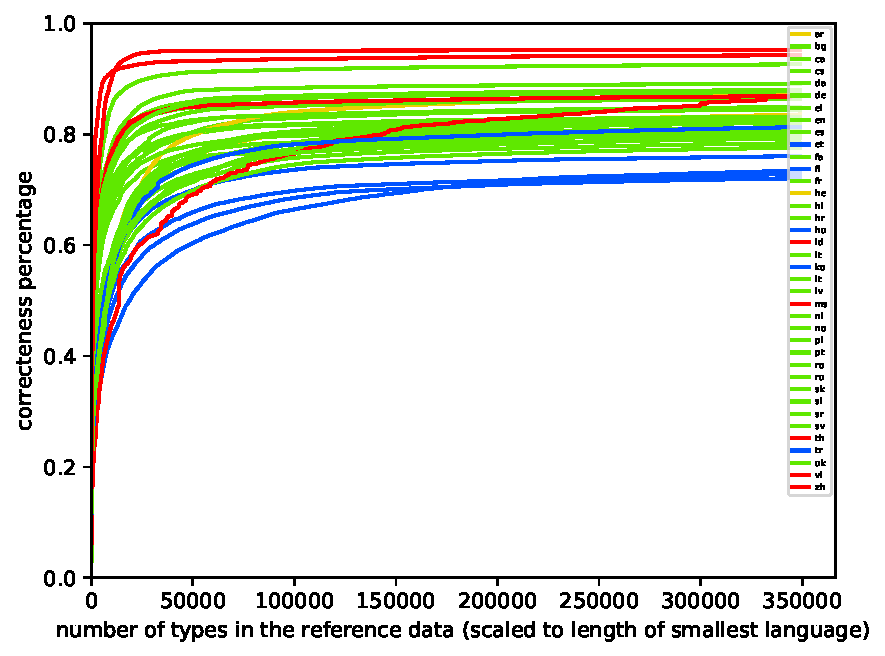
\includegraphics[width=\textwidth]{graphs/nas/morph_types/norm_huge_type_token_performance}
    \end{subfigure}
    \begin{subfigure}[b]{0.32\textwidth}
    	\centering
        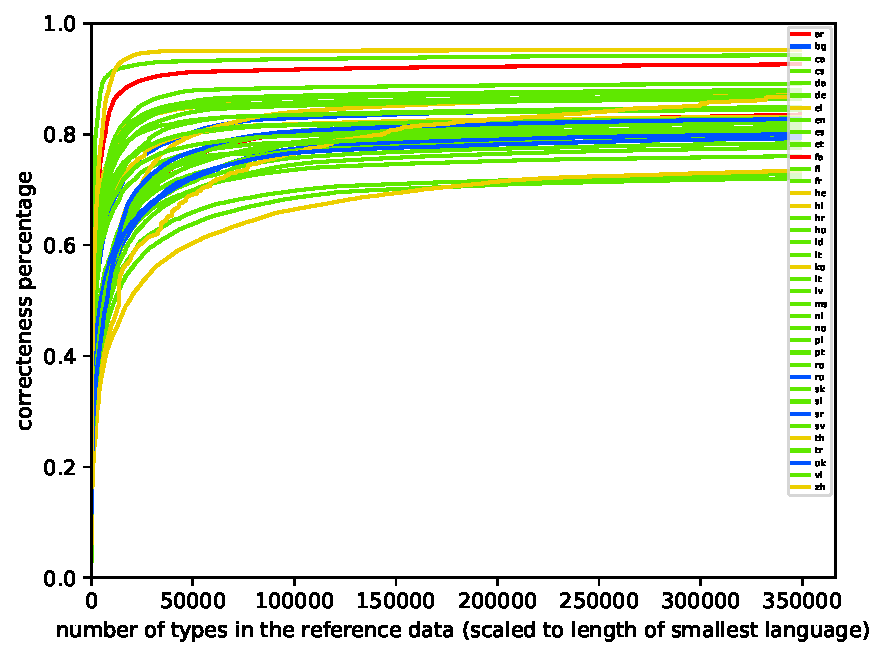
\includegraphics[width=\textwidth]{graphs/nas/scripts/norm_huge_type_token_performance}
    \end{subfigure}
    \caption{The correctness percentage for NAS, first colored individually, then by script (green is fusional, blue is agglutinative, red is isolating and yellow is introflexive) and by type (green is Latin, blue is Cyrillic, red is Arabic and yellow are others).}
	\label{Figure:nas_norm_huge_type_token_performance}
\end{figure}

The corresponding graphs can be found in Figure \ref{Figure:nas_norm_huge_type_token_performance}. A table showing the end results can be found in Table \

The general range of the correctness percentages over all languages is between 75\% and 95\%. The lowest performing languages are Finnish, Estonian, and Korean. The highest performing languages are Chinese, Vietnamese, and Farsi. The remaining languages are fairly close together, ranging between 79\% and 91\%. There is a fairly clear picture in terms of morphological types, with the agglutinative languages having some of the lowest correctness percentages and isolating languages having some of the highest. This is to be expected as agglutinative languages tend to string a high number of morphemes together into a single word, resulting in many different possibilities for words, only few of which exist or have been observed, while isolating languages only have one morpheme per word, which results in few different words overall and thus an easier task for the language model. The fusional and introflexive languages all have average performance compared to the other models. In terms of scripts used, there is no clear correlation between any of the scripts and the performance, except, possibly that the languages using Cyrillic are very close together.
\subsubsection{GRU}

\begin{figure}[h]
    \centering
    \begin{subfigure}[b]{0.32\textwidth}
    	\centering
        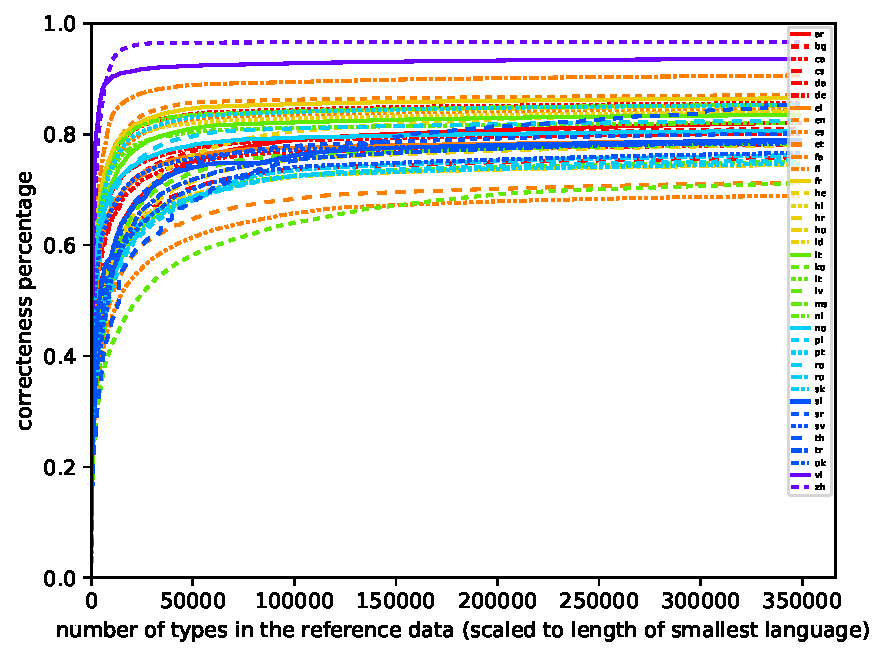
\includegraphics[width=\textwidth]{graphs/gru/norm_huge_type_token_performance}
    \end{subfigure}
    \begin{subfigure}[b]{0.32\textwidth}
    	\centering
        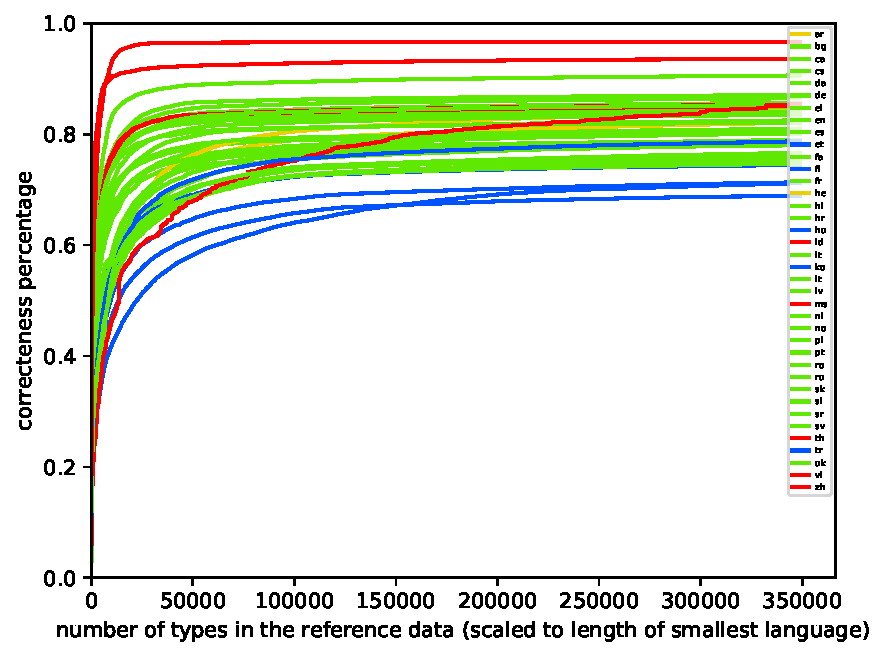
\includegraphics[width=\textwidth]{graphs/gru/morph_types/norm_huge_type_token_performance}
    \end{subfigure}
    \begin{subfigure}[b]{0.32\textwidth}
    	\centering
        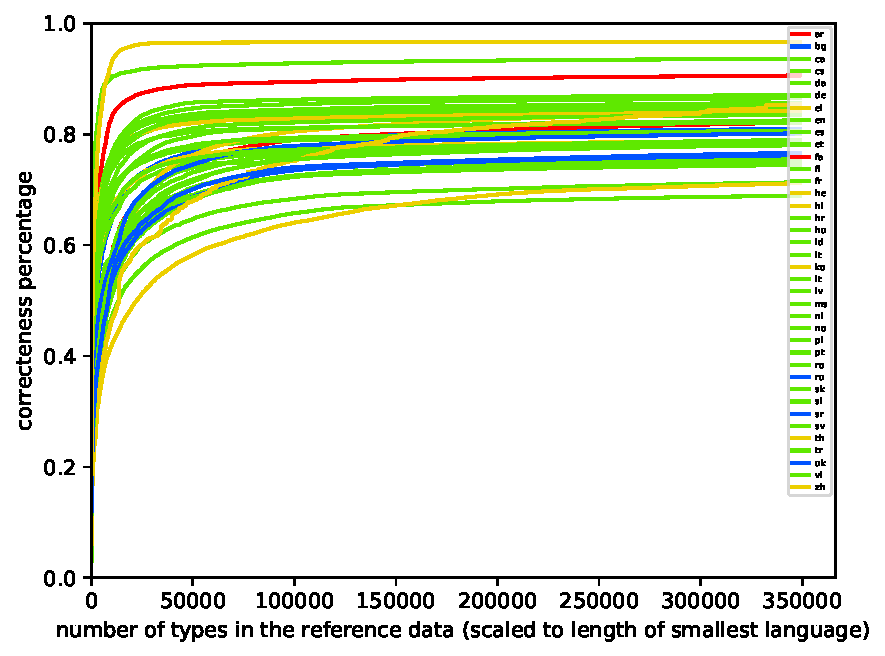
\includegraphics[width=\textwidth]{graphs/gru/scripts/norm_huge_type_token_performance}
    \end{subfigure}
    \caption{The correctness percentage for GRU, first colored individually, then by script (green is fusional, blue is agglutinative, red is isolating and yellow is introflexive) and by type (green is Latin, blue is Cyrillic, red is Arabic and yellow are others).}
	\label{Figure:gru_norm_huge_type_token_performance}
\end{figure}

The corresponding graphs can be found in Figure \ref{Figure:gru_norm_huge_type_token_performance}.

The general range of the correctness percentages for GRU is similar to NAS: between 72\% and 96\%. The lower performing languages, as for NAS, are Finnish, Estonian, and Korean, and the highest performing languages are Chinese, Vietnamese, and Farsi. The remaining languages range between 77\% and 89\%. In terms of morphology types, the picture is also similar, with the agglutinative languages performing worst and the isolating languages best, with the fusional and introflexive languages in the middle. Again, the Cyrillic languages are close together in the middle of the language range. 
\subsubsection{RNN}

\begin{figure}[h]
    \centering
    \begin{subfigure}[b]{0.32\textwidth}
    	\centering
        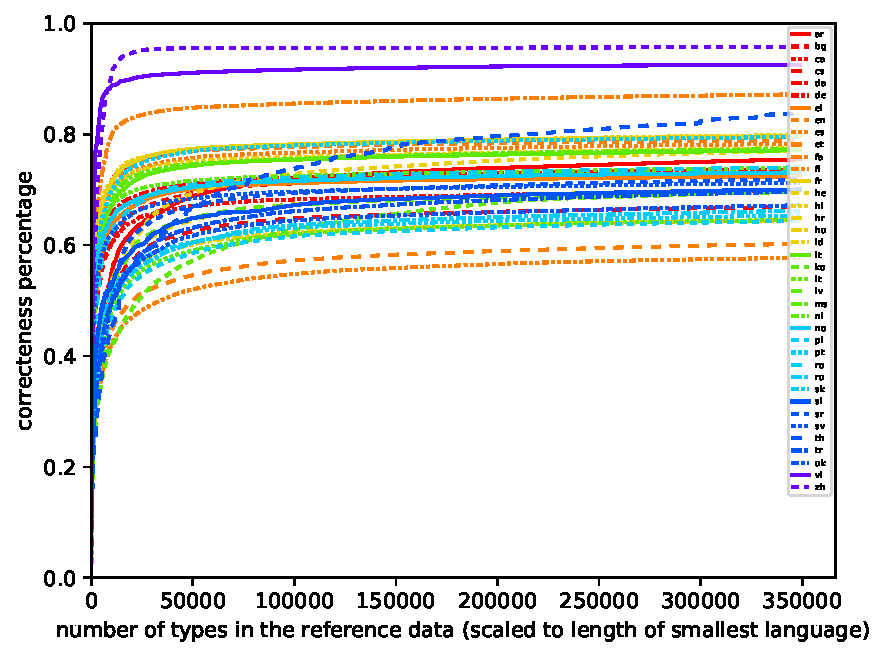
\includegraphics[width=\textwidth]{graphs/rnn/norm_huge_type_token_performance}
    \end{subfigure}
    \begin{subfigure}[b]{0.32\textwidth}
    	\centering
        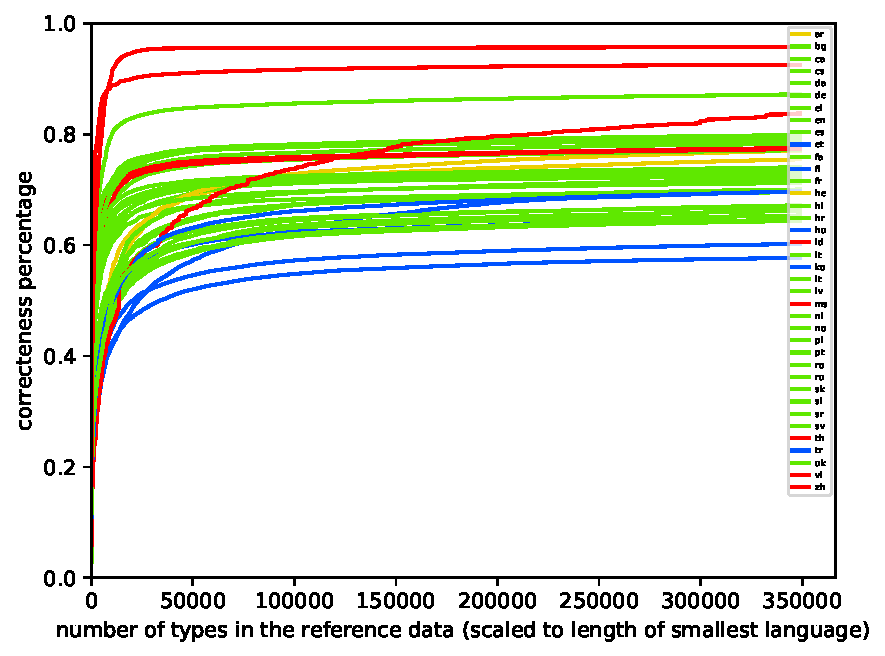
\includegraphics[width=\textwidth]{graphs/rnn/morph_types/norm_huge_type_token_performance}
    \end{subfigure}
    \begin{subfigure}[b]{0.32\textwidth}
    	\centering
        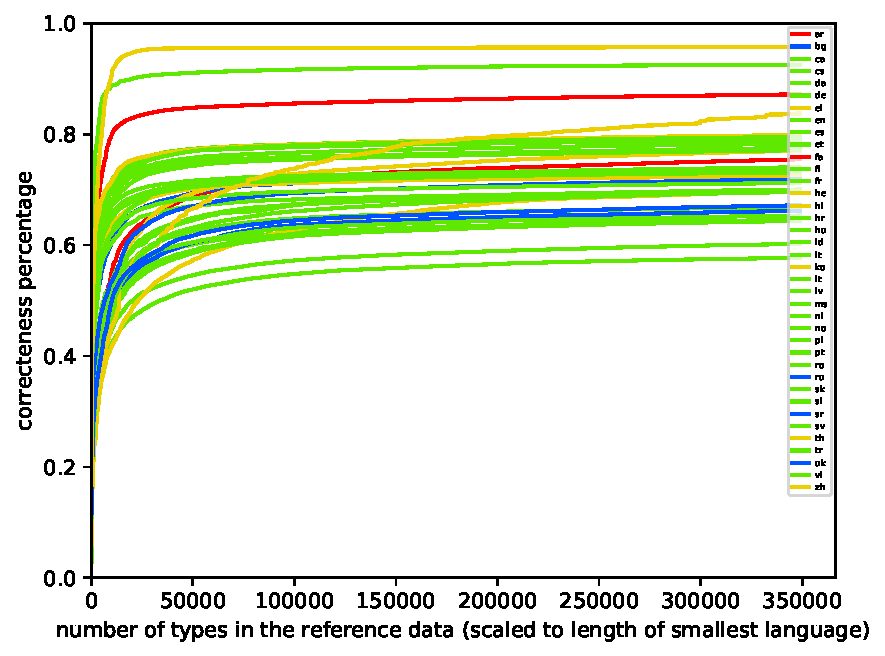
\includegraphics[width=\textwidth]{graphs/rnn/scripts/norm_huge_type_token_performance}
    \end{subfigure}
    \caption{The correctness percentage for RNN, first colored individually, then by script (green is fusional, blue is agglutinative, red is isolating and yellow is introflexive) and by type (green is Latin, blue is Cyrillic, red is Arabic and yellow are others).}
	\label{Figure:rnn_norm_huge_type_token_performance}
\end{figure}

The corresponding graphs can be found in Figure \ref{Figure:rnn_norm_huge_type_token_performance}.

The correctness percentages for RNN are both lower and more spread out than the ones for NAS and GRU, ranging between 62\% and 95\%. The lowest performing languages, as previously, are Finnish and Estonian, while the highest performing languages are Chinese, Vietnamese, Farsi, and Thai. The behaviour of Thai is somewhat pecular: it increases performance with the size of the reference data far more quickly than any of the other languages. The remaining languages range between 60\% and 80\%. In terms of morphology types, as for NAS and GRU, agglutinative languages perform well in general, while isolating languages perform among the worst. 

\subsubsection{LSTM}

\begin{figure}[h]
    \centering
    \begin{subfigure}[b]{0.32\textwidth}
    	\centering
        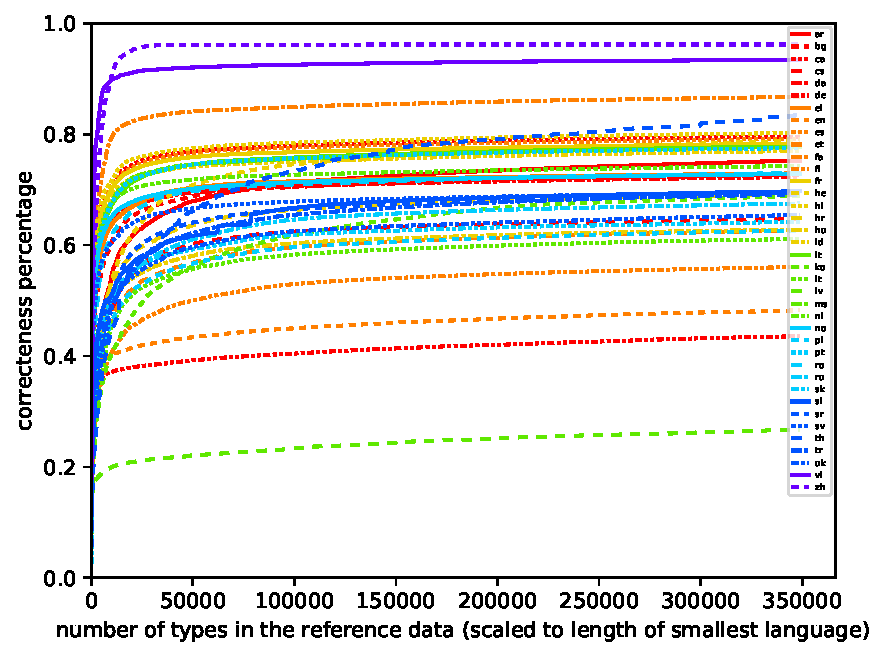
\includegraphics[width=\textwidth]{graphs/lstm/norm_huge_type_token_performance}
    \end{subfigure}
    \begin{subfigure}[b]{0.32\textwidth}
    	\centering
        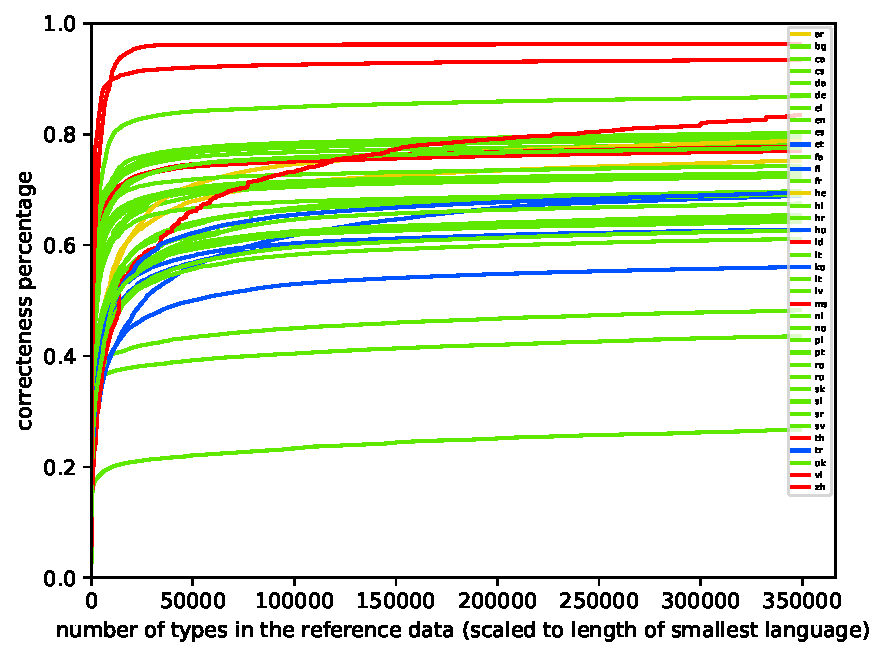
\includegraphics[width=\textwidth]{graphs/lstm/morph_types/norm_huge_type_token_performance}
    \end{subfigure}
    \begin{subfigure}[b]{0.32\textwidth}
    	\centering
        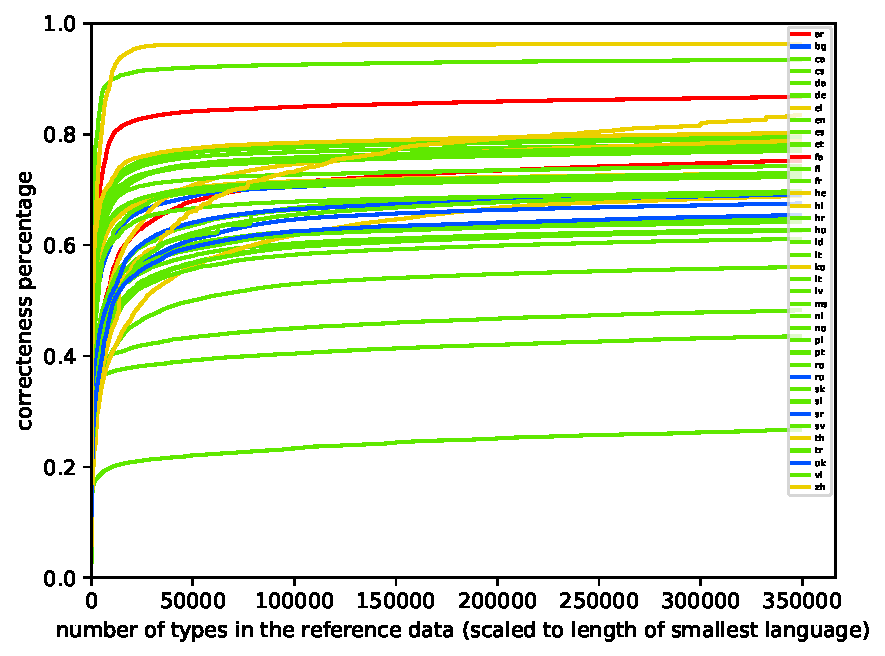
\includegraphics[width=\textwidth]{graphs/lstm/scripts/norm_huge_type_token_performance}
    \end{subfigure}
    \caption{The correctness percentage for LSTM, first colored individually, then by script (green is fusional, blue is agglutinative, red is isolating and yellow is introflexive) and by type (green is Latin, blue is Cyrillic, red is Arabic and yellow are others).}
	\label{Figure:lstm_norm_huge_type_token_performance}
\end{figure}

The corresponding graphs can be found in Figure \ref{Figure:lstm_norm_huge_type_token_performance}.

The correctness percentages for LSTM are even more spread out and are generally worse than those for RNN, ranging from 26\% to 96\%. The lowest performing languages are also different: Latvian, German, English, and Finnish. The highest performing languages are Chinese, Vietnamese, Farsi, and Thai. The remaining languages range between 61\% and 80\%, similar to RNN. The picture with regards to both morphology types and scripts is far less obvious than for the other three models, as the lowest performing languages are fusional and use Latin, which leads to there being no clear correlation between the performance and scripts or morphological types.

\subsection{New sensible word count}
While we mainly evaluated the absolute values for correctness percentages, this is less simple for the new sensible word count. As can be seen quickly from GRAPH, we also need to consider the slope of every language’s line and the point at which it suddenly becomes steeper. The most probable reason for this breaking point is that on the x-axis, we count the number of types in the reference data. Presumably, the turning point occurs once most common and simple words have already occurred and the more complicated words, which are more likely to have been generated by the language model, start appearing. 
In general, LSTM and RNN perform better than NAS and GRU for the new sensible word count. Also, languages with an earlier turning point have shallower slopes, and languages with a later turning point have steeper slopes. These slopes are very relevant because high differences in slope mean that the order of the languages can change significantly with increased reference data.  Introflexive and agglutinative languages tend to perform better than average while isolating languages perform worse then average.

\subsubsection{NAS}
\begin{figure}[h]
    \centering
    \begin{subfigure}[b]{0.32\textwidth}
    	\centering
        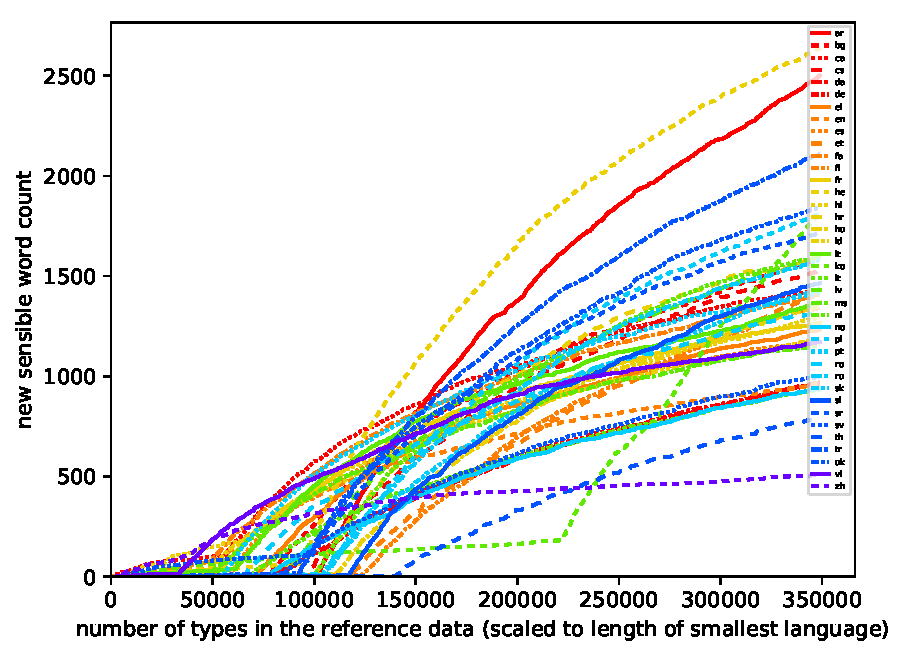
\includegraphics[width=\textwidth]{graphs/nas/norm_huge_type_type_performance}
    \end{subfigure}
    \begin{subfigure}[b]{0.32\textwidth}
    	\centering
        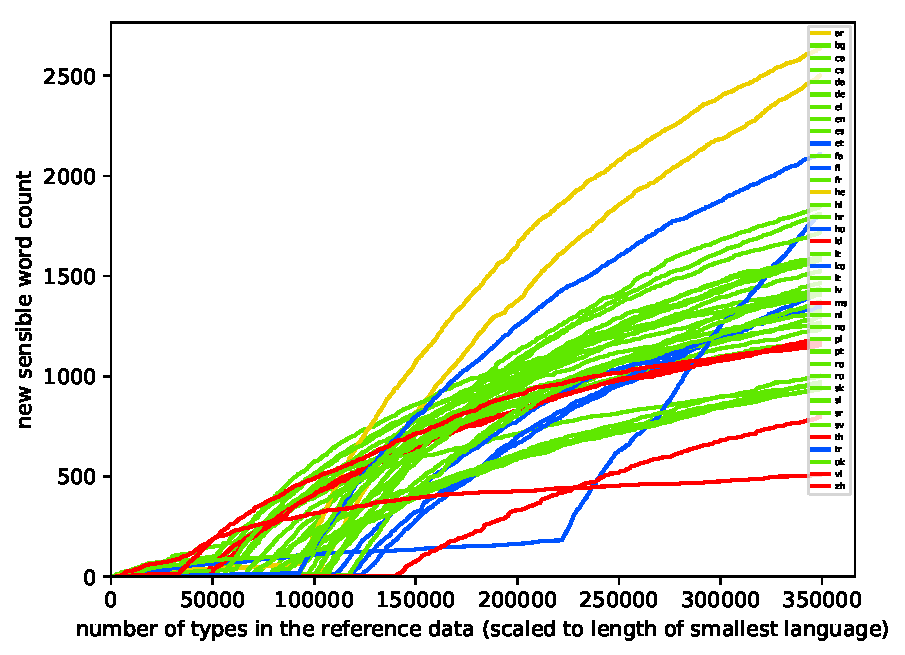
\includegraphics[width=\textwidth]{graphs/nas/morph_types/norm_huge_type_type_performance}
    \end{subfigure}
    \begin{subfigure}[b]{0.32\textwidth}
    	\centering
        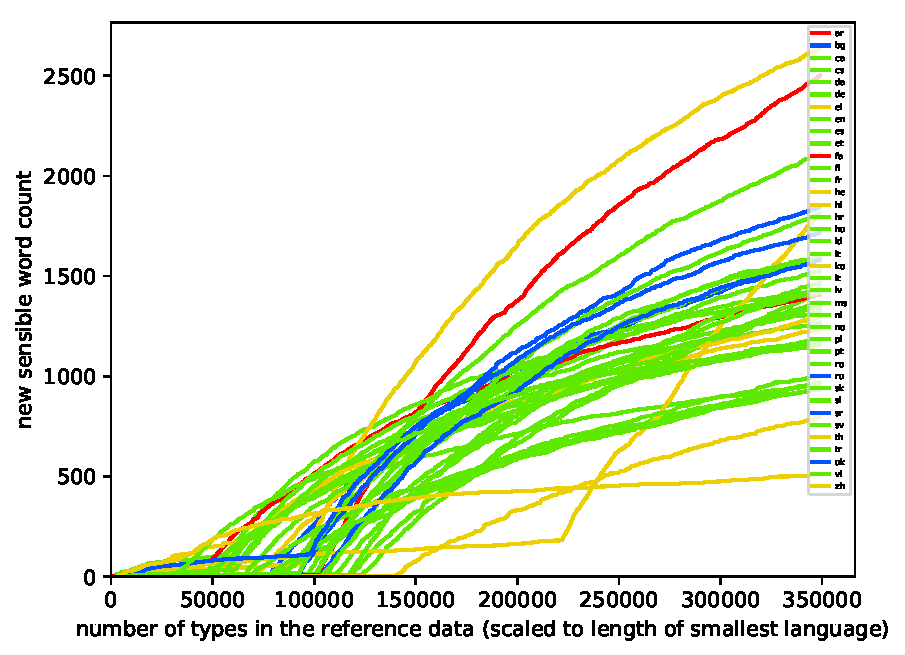
\includegraphics[width=\textwidth]{graphs/nas/scripts/norm_huge_type_type_performance}
    \end{subfigure}
    \caption{The new sensible word count for NAS, first colored individually, then by script (green is fusional, blue is agglutinative, red is isolating and yellow is introflexive) and by type (green is Latin, blue is Cyrillic, red is Arabic and yellow are others).}
	\label{Figure:nas_norm_huge_type_type_performance}
\end{figure}

The corresponding graph can be found in Figure \ref{Figure:nas_norm_huge_type_type_performance}.

The new sensible word counts for NAS range between 500 and 3000 words. It should however be noted that those numbers rise steeply with the size of the reference data, so they should not be taken as an absolute value. The worst performing languages are Chinese and Thai, and the best performing languages are Hebrew, Arabic, Korean, and Turkish. The languages with the steepest slopes are generally the best performing ones, while the ones with the shallowest slopes are the worst performing ones. Generally, languages with a late turning point tend to have a steeper slope, while languages with an earlier turning point tend to have a shallower slope. Some exceptions to this are Hebrew and Korean. In terms of morphological types, introflexive and agglutinative languages have some of the best performances, while isolating languages are amongst the lowest performing ones. Presumably, this is because it is harder to generate new words in isolating languages, as words consist of only a single morpheme, and easier in agglutinative languages, as the morphemes are simply strung together. In terms of scripts, the only distinguishable pattern is that languages using Cyrillic perform rather better than average, although there is no apparent explanation for this. 
\subsubsection{GRU}


\begin{figure}[h]
    \centering
    \begin{subfigure}[b]{0.32\textwidth}
    	\centering
        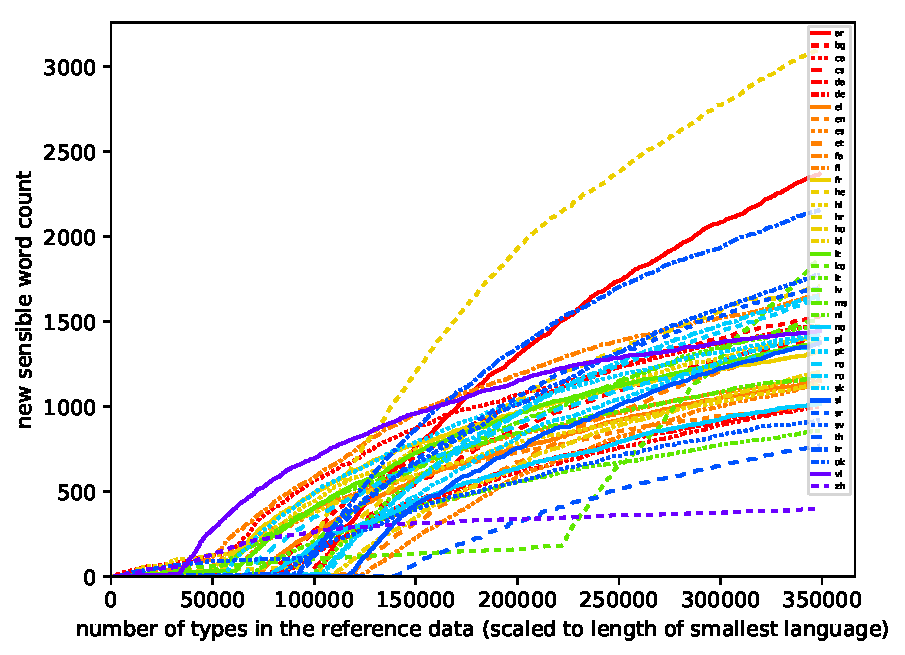
\includegraphics[width=\textwidth]{graphs/gru/norm_huge_type_type_performance}
    \end{subfigure}
    \begin{subfigure}[b]{0.32\textwidth}
    	\centering
        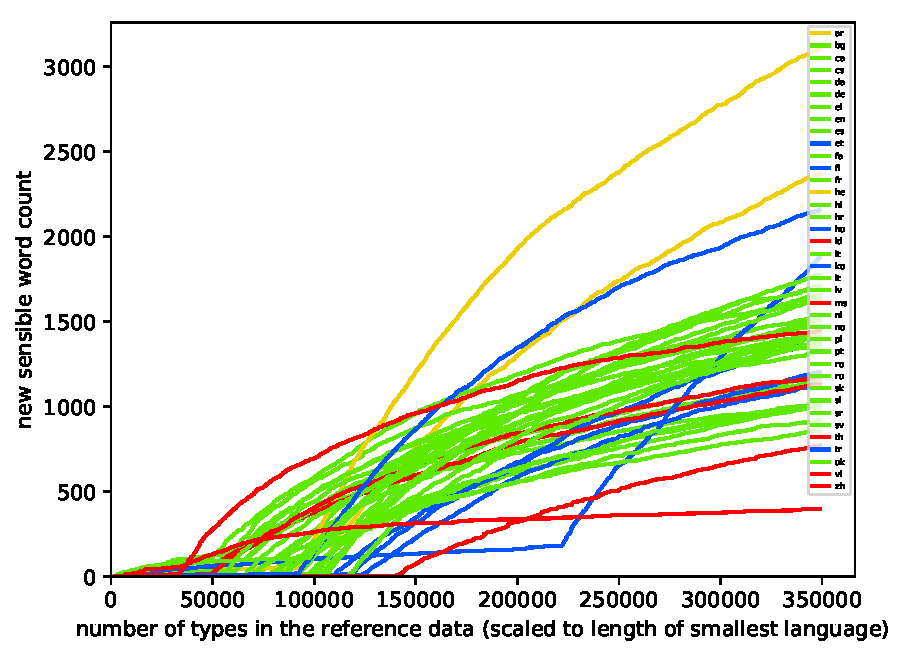
\includegraphics[width=\textwidth]{graphs/gru/morph_types/norm_huge_type_type_performance}
    \end{subfigure}
    \begin{subfigure}[b]{0.32\textwidth}
    	\centering
        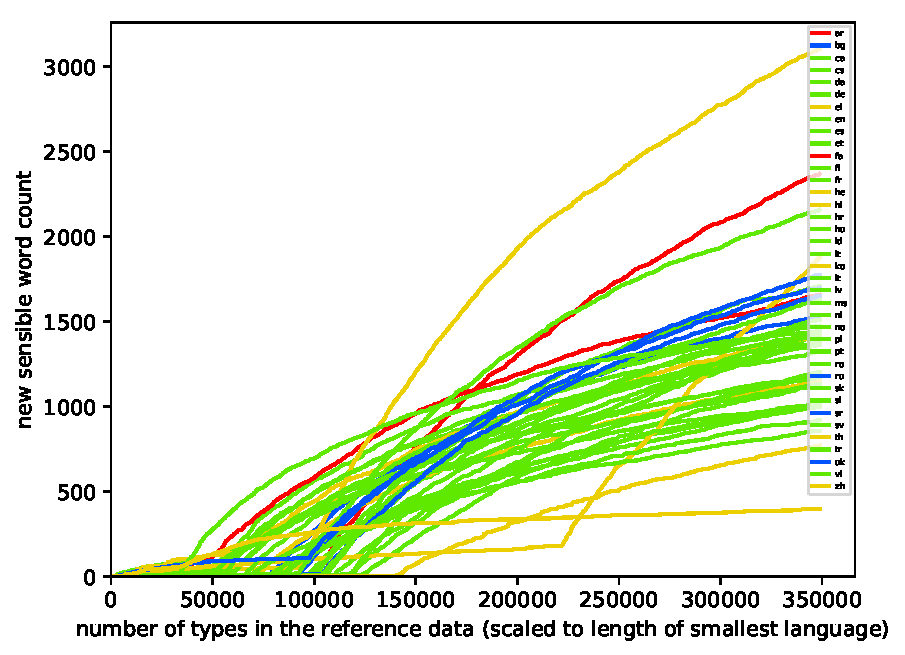
\includegraphics[width=\textwidth]{graphs/gru/scripts/norm_huge_type_type_performance}
    \end{subfigure}
    \caption{The new sensible word count for GRU, first colored individually, then by script (green is fusional, blue is agglutinative, red is isolating and yellow is introflexive) and by type (green is Latin, blue is Cyrillic, red is Arabic and yellow are others).}
	\label{Figure:gru_norm_huge_type_type_performance}
\end{figure}

The corresponding graph can be found in Figure \ref{Figure:gru_norm_huge_type_type_performance}.

The new sensible word counts for GRU are very similar to those for NAS, with the exception of the much improved performance of Hebrew. The counts range between 500 and 3000 new words. The best performing languages are Hebrew, Arabic, Turkish, and Korean, while the worst performing languages are Chinese, Thai, and Dutch. The picture in terms of morphological types is also similar, with introflexive and agglutinative languages performing better than average, and isolating language performing worse than average.

\subsubsection{RNN}

\begin{figure}[h]
    \centering
    \begin{subfigure}[b]{0.32\textwidth}
    	\centering
        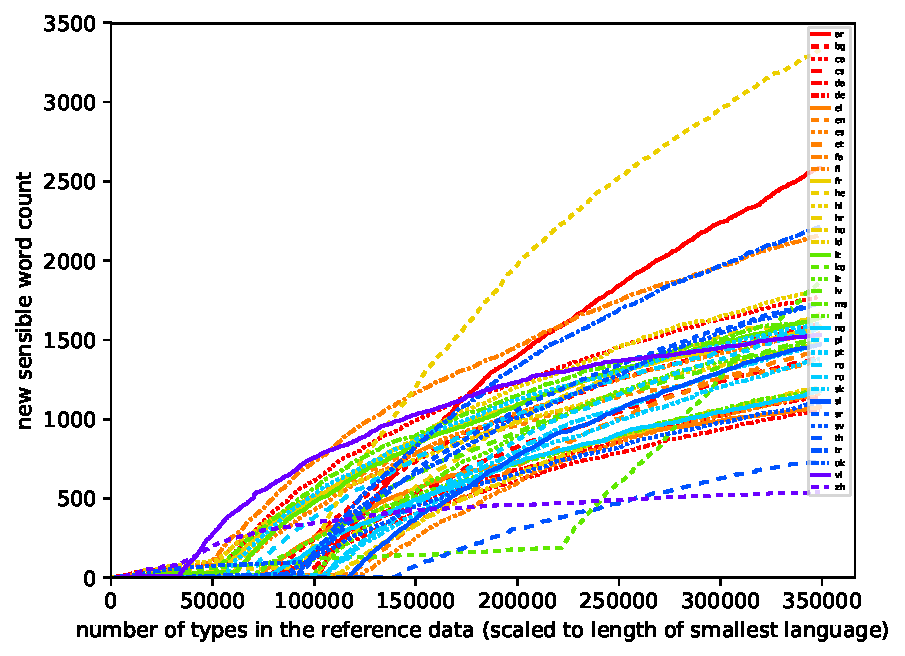
\includegraphics[width=\textwidth]{graphs/rnn/norm_huge_type_type_performance}
    \end{subfigure}
    \begin{subfigure}[b]{0.32\textwidth}
    	\centering
        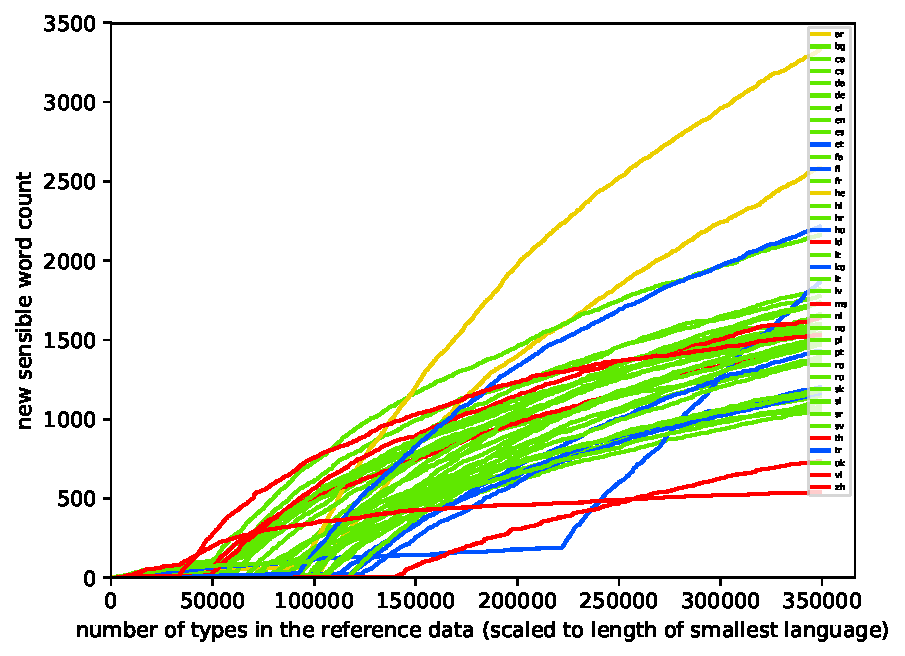
\includegraphics[width=\textwidth]{graphs/rnn/morph_types/norm_huge_type_type_performance}
    \end{subfigure}
    \begin{subfigure}[b]{0.32\textwidth}
    	\centering
        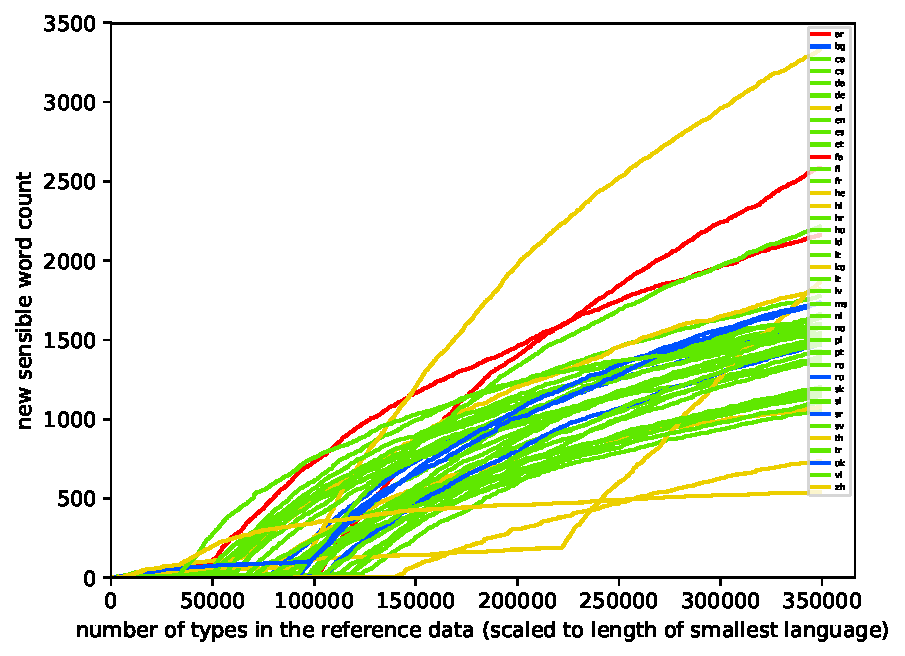
\includegraphics[width=\textwidth]{graphs/rnn/scripts/norm_huge_type_type_performance}
    \end{subfigure}
    \caption{The new sensible word count for RNN, first colored individually, then by script (green is fusional, blue is agglutinative, red is isolating and yellow is introflexive) and by type (green is Latin, blue is Cyrillic, red is Arabic and yellow are others).}
	\label{Figure:rnn_norm_huge_type_type_performance}
\end{figure}

The corresponding graph can be found in Figure \ref{Figure:rnn_norm_huge_type_type_performance}.

The new sensible word counts for RNN are generally higher than those for the last two models discussed, ranging between 500 and 3500 words. The best performing languages are Hebrew, Arabic, Turkish, Farsi, and Korean. The worst performing languages are Chinese and Thai. This order is similar to the other models, as is the picture in terms of turning points and slopes. Interestingly, there is a much less clear picture in terms of morphological types, as isolating and agglutinative languages perform equally well in general, while the two introflexive languages investigated are still the best performing ones. Regarding scripts, languages using Cyrillic perform rather better than average, similarly to the other models. 

\subsubsection{LSTM}

\begin{figure}[h]
    \centering
    \begin{subfigure}[b]{0.32\textwidth}
    	\centering
        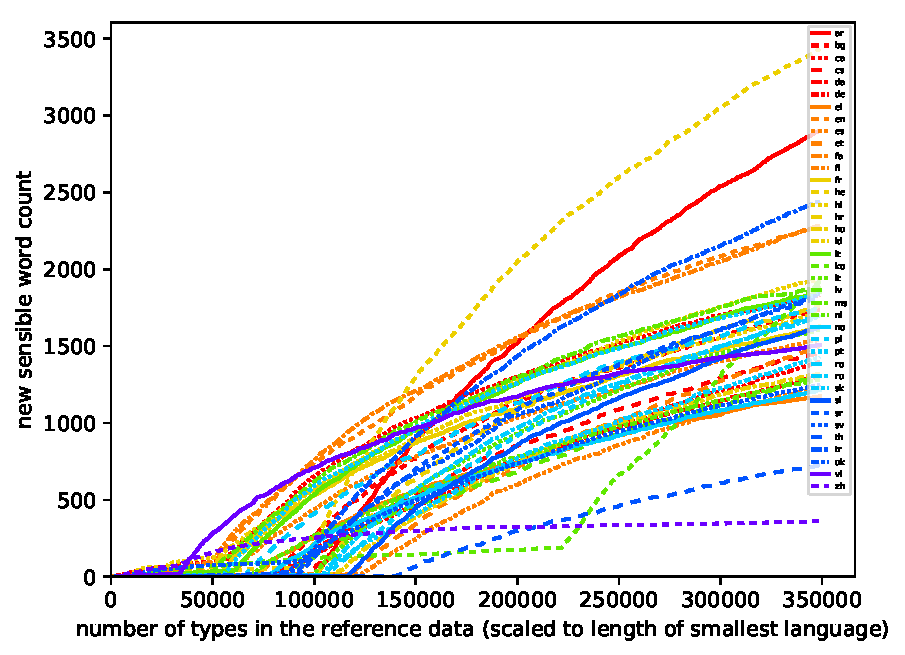
\includegraphics[width=\textwidth]{graphs/lstm/norm_huge_type_type_performance}
    \end{subfigure}
    \begin{subfigure}[b]{0.32\textwidth}
    	\centering
        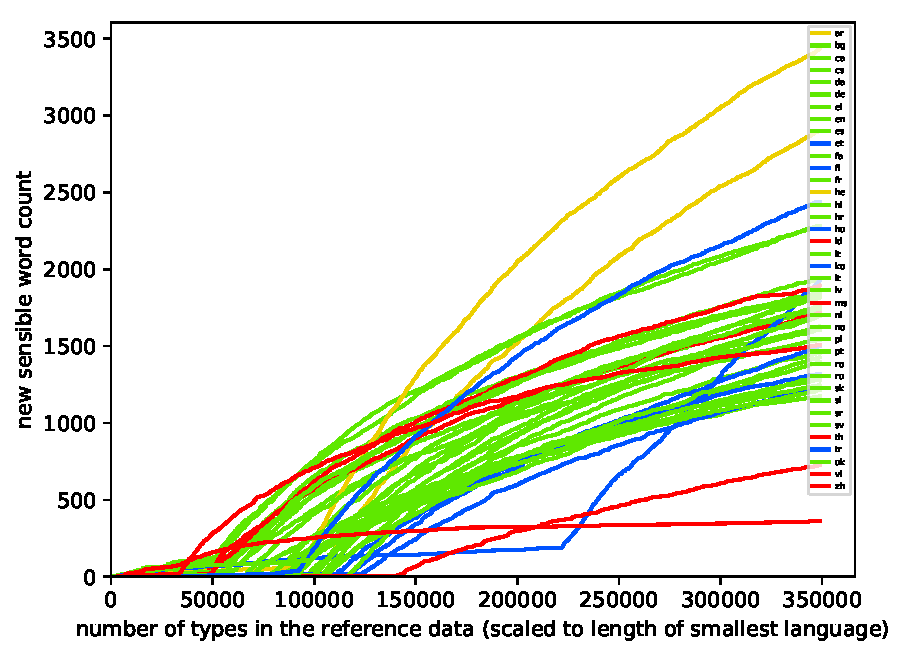
\includegraphics[width=\textwidth]{graphs/lstm/morph_types/norm_huge_type_type_performance}
    \end{subfigure}
    \begin{subfigure}[b]{0.32\textwidth}
    	\centering
        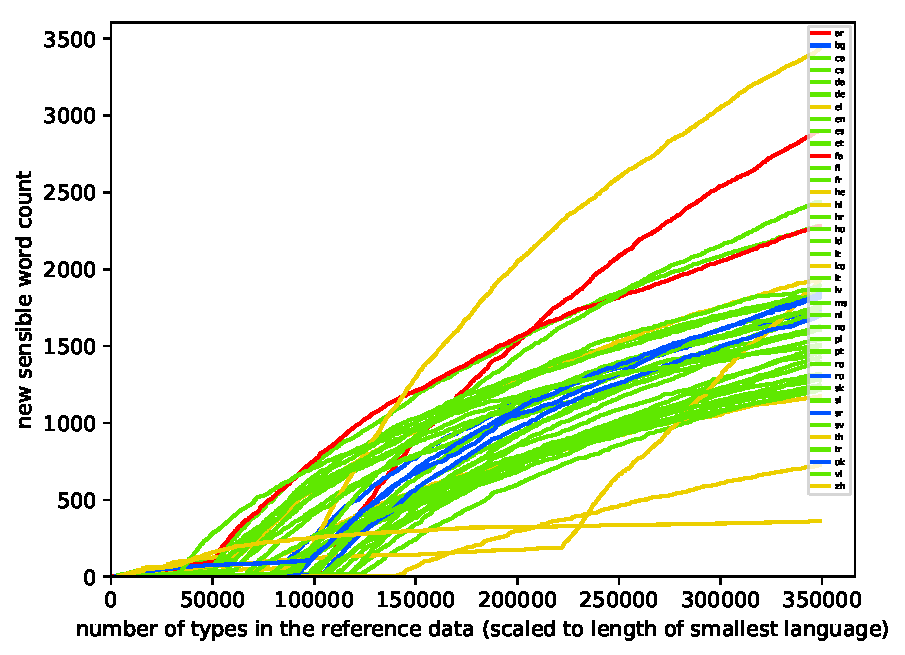
\includegraphics[width=\textwidth]{graphs/lstm/scripts/norm_huge_type_type_performance}
    \end{subfigure}
    \caption{The new sensible word count for LSTM, first colored individually, then by script (green is fusional, blue is agglutinative, red is isolating and yellow is introflexive) and by type (green is Latin, blue is Cyrillic, red is Arabic and yellow are others).}
	\label{Figure:lstm_norm_huge_type_type_performance}
\end{figure}

The corresponding graph can be found in Figure \ref{Figure:lstm_norm_huge_type_type_performance}.

The new sensible word counts for LSTM are very similar to those for RNN, also ranging between 500 and 3500 new words. The best performing languages are Hebrew, Arabic, Turkish, English, Farsi, and Korean, while the worst performing languages are Chinese and Thai. This order is identical to the one in RNN, except for English, which improved significantly. Similarly to RNN, there is also no clear picture in terms of morphological types or scripts used. 

\begin{table}[h]
\centering
\caption{Performance values for RNN (reference data adjusted to size of smallest language)}
\label{table:rnn}
\begin{tabular}{lrr}
\textbf{Language} & \textbf{New sensible word count} & \textbf{Correctness percentage} \\ \hline \hline
da & 1146 & 73.63\% \\ \hline
lt & 1491 & 64.58\% \\ \hline
pl & 1578 & 64.39\% \\ \hline
en & 1365 & 78.91\% \\ \hline
sk & 1380 & 65.35\% \\ \hline
ro & 1581 & 74.04\% \\ \hline
lv & 1514 & 69.59\% \\ \hline
fi & 1163 & 57.72\% \\ \hline
pt & 1601 & 79.51\% \\ \hline
it & 1638 & 77.12\% \\ \hline
ms & 1642 & 77.32\% \\ \hline
ru & 1469 & 66.17\% \\ \hline
nl & 1185 & 73.94\% \\ \hline
fa & 2161 & 87.20\% \\ \hline
et & 1430 & 60.22\% \\ \hline
hu & 1200 & 64.50\% \\ \hline
bg & 1600 & 73.21\% \\ \hline
vi & 1530 & 92.54\% \\ \hline
fr & 1584 & 79.68\% \\ \hline
hi & 1818 & 79.86\% \\ \hline
el & 1075 & 72.40\% \\ \hline
tr & 2215 & 69.70\% \\ \hline
ca & 1776 & 79.63\% \\ \hline
th & 737 & 83.75\% \\ \hline
sl & 1471 & 70.03\% \\ \hline
uk & 1734 & 67.19\% \\ \hline
sv & 1102 & 71.21\% \\ \hline
he & 3330 & 77.06\% \\ \hline
sr & 1735 & 71.85\% \\ \hline
zh & 541 & 95.68\% \\ \hline
ar & 2584 & 75.48\% \\ \hline
no & 1178 & 73.14\% \\ \hline
id & 1475 & 77.52\% \\ \hline
de & 1061 & 69.83\% \\ \hline
es & 1541 & 78.26\% \\ \hline
ko & 1861 & 69.75\% \\ \hline
hr & 1661 & 70.01\% \\ \hline
cs & 1394 & 66.89\% \\
\end{tabular}
\end{table}




\begin{table}[h]
\centering
\caption{Performance values for LSTM (reference data adjusted to size of smallest language)}
\label{table:lstm}
\begin{tabular}{lrr}
\textbf{Language} & \textbf{New sensible word count} & \textbf{Correctness percentage} \\ \hline \hline
da & 1301 & 72.31\% \\ \hline
lt & 1607 & 61.10\% \\ \hline
pl & 1698 & 62.63\% \\ \hline
en & 2280 & 48.23\% \\ \hline
sk & 1428 & 64.23\% \\ \hline
ro & 1748 & 73.00\% \\ \hline
lv & 1299 & 26.75\% \\ \hline
fi & 1218 & 56.03\% \\ \hline
pt & 1842 & 77.52\% \\ \hline
it & 1850 & 77.80\% \\ \hline
ms & 1893 & 77.72\% \\ \hline
ru & 1700 & 67.52\% \\ \hline
nl & 1280 & 74.26\% \\ \hline
fa & 2282 & 86.75\% \\ \hline
et & 1499 & 62.71\% \\ \hline
hu & 1320 & 62.78\% \\ \hline
bg & 1739 & 72.70\% \\ \hline
vi & 1505 & 93.41\% \\ \hline
fr & 1627 & 78.30\% \\ \hline
hi & 1934 & 80.22\% \\ \hline
el & 1173 & 72.94\% \\ \hline
tr & 2440 & 69.45\% \\ \hline
ca & 1830 & 79.58\% \\ \hline
th & 729 & 83.42\% \\ \hline
sl & 1622 & 69.72\% \\ \hline
uk & 1840 & 65.45\% \\ \hline
sv & 1248 & 69.55\% \\ \hline
he & 3434 & 78.81\% \\ \hline
sr & 1816 & 69.11\% \\ \hline
zh & 360 & 96.22\% \\ \hline
ar & 2899 & 75.27\% \\ \hline
no & 1215 & 72.85\% \\ \hline
id & 1717 & 77.03\% \\ \hline
de & 1396 & 43.61\% \\ \hline
es & 1539 & 79.16\% \\ \hline
ko & 1923 & 68.89\% \\ \hline
hr & 1761 & 69.13\% \\ \hline
cs & 1459 & 64.71\% \\ 
\end{tabular}
\end{table}




\begin{table}[h]
\centering
\caption{Performance values for NAS (reference data adjusted to size of smallest language)}
\label{table:nas}
\begin{tabular}{lrr}
\textbf{Language} & \textbf{New sensible word count} & \textbf{Correctness percentage} \\ \hline \hline
da & 960 & 82.78\% \\ \hline
lt & 1599 & 78.36\% \\ \hline
pl & 1810 & 77.60\% \\ \hline
en & 966 & 89.14\% \\ \hline
sk & 1437 & 79.25\% \\ \hline
ro & 1325 & 84.91\% \\ \hline
lv & 1588 & 82.09\% \\ \hline
fi & 1344 & 72.05\% \\ \hline
pt & 1415 & 87.79\% \\ \hline
it & 1372 & 86.45\% \\ \hline
ms & 1156 & 86.88\% \\ \hline
ru & 1580 & 80.04\% \\ \hline
nl & 935 & 84.45\% \\ \hline
fa & 1406 & 92.62\% \\ \hline
et & 1415 & 72.87\% \\ \hline
hu & 1350 & 76.05\% \\ \hline
bg & 1581 & 84.78\% \\ \hline
vi & 1172 & 94.26\% \\ \hline
fr & 1267 & 87.69\% \\ \hline
hi & 1296 & 86.66\% \\ \hline
el & 1233 & 83.19\% \\ \hline
tr & 2108 & 81.29\% \\ \hline
ca & 1429 & 87.62\% \\ \hline
th & 798 & 86.92\% \\ \hline
sl & 1464 & 81.31\% \\ \hline
uk & 1844 & 79.29\% \\ \hline
sv & 1001 & 80.96\% \\ \hline
he & 2634 & 87.05\% \\ \hline
sr & 1718 & 82.75\% \\ \hline
zh & 509 & 95.17\% \\ \hline
ar & 2500 & 83.56\% \\ \hline
no & 939 & 82.81\% \\ \hline
id & 1187 & 86.68\% \\ \hline
de & 970 & 79.87\% \\ \hline
es & 1173 & 87.97\% \\ \hline
ko & 1803 & 73.45\% \\ \hline
hr & 1600 & 82.88\% \\ \hline
cs & 1523 & 80.50\% \\ 
\end{tabular}
\end{table}




\begin{table}[h]
\centering
\caption{Performance values for GRU (reference data adjusted to size of smallest language)}
\label{table:gru}
\begin{tabular}{lrr}
\textbf{Language} & \textbf{New sensible word count} & \textbf{Correctness percentage} \\ \hline \hline
da & 1014 & 80.13\% \\ \hline
lt & 1476 & 75.00\% \\ \hline
pl & 1635 & 75.33\% \\ \hline
en & 1014 & 87.07\% \\ \hline
sk & 1421 & 74.67\% \\ \hline
ro & 1362 & 82.49\% \\ \hline
lv & 1510 & 78.34\% \\ \hline
fi & 1124 & 68.91\% \\ \hline
pt & 1423 & 85.30\% \\ \hline
it & 1377 & 83.53\% \\ \hline
ms & 1178 & 85.36\% \\ \hline
ru & 1653 & 76.22\% \\ \hline
nl & 859 & 82.11\% \\ \hline
fa & 1658 & 90.61\% \\ \hline
et & 1391 & 71.34\% \\ \hline
hu & 1205 & 74.49\% \\ \hline
bg & 1533 & 80.97\% \\ \hline
vi & 1447 & 93.61\% \\ \hline
fr & 1325 & 86.50\% \\ \hline
hi & 1417 & 84.02\% \\ \hline
el & 1150 & 78.85\% \\ \hline
tr & 2158 & 78.72\% \\ \hline
ca & 1474 & 85.65\% \\ \hline
th & 772 & 85.45\% \\ \hline
sl & 1377 & 78.97\% \\ \hline
uk & 1777 & 76.65\% \\ \hline
sv & 920 & 78.37\% \\ \hline
he & 3105 & 84.21\% \\ \hline
sr & 1700 & 80.16\% \\ \hline
zh & 398 & 96.64\% \\ \hline
ar & 2369 & 82.11\% \\ \hline
no & 1018 & 80.62\% \\ \hline
id & 1134 & 85.13\% \\ \hline
de & 998 & 78.09\% \\ \hline
es & 1176 & 84.65\% \\ \hline
ko & 1877 & 71.19\% \\ \hline
hr & 1709 & 78.03\% \\ \hline
cs & 1422 & 75.77\% \\
\end{tabular}
\end{table}


\chapter{Conclusion and Future Work}
\section{Conclusion}
This thesis has introduced two metrics for measuring the performance of character-level language models and evaluated four variants of character-level recurrent neural networks used on 38 languages. We introduced correctness percentage, which is a measure for how many of the words output by the model are real words, and new sensible word count, which is a measure for how many real words the model generates that it has not observed during training. The correctness percentage assesses how great the disadvantage compared to word-level models is, because it measures how many non-words the character-level model produces, and the new sensible word count assesses how great the advantage over word-level models is because it measures how many correct words the model was able to generate by learning about morphology. Together, these metrics measure how well character-level models perform compared to word-level models. 

Using these metrics, we assess a simple recurrent neural network, a long-short-term memory network, a recurrent neural network using gated recurrent units and one using a cell generated by neural architecture search. We find that for most languages, there is a trade-off between the models: if one model performs best in one metric, it performs worst in the other, and vice versa. The most common pattern for correctness percentages is that NAS performs best, followed by GRU, then RNN and then LSTM. For most languages, correctness percentages range between 70\% and 80\%, which means that at least 20\% of all output words do not exist. This figure could be decreased somewhat with increased reference data, but the difference will not be significant. The most common pattern for new sensible word count is that LSTM performs best, followed by RNN, then GRU and then NAS. For many languages, there is this exact trade-off, which means the choice of model will depend on the user’s priorities, but for many others, we give recommendations  - for example, that NAS is often better than GRU in both metrics, or that LSTM is always better than RNN. This suggests that in general, NAS and GRU are better at memorizing words, while LSTM and RNN are better at recognizing patterns within the words. This is especially interesting since NAS and GRU are the newer models, recognized as an improvement over their predecessors, but they do not categorically perform better for character-level language modelling. When comparing the performances of the languages against each other, agglutinative and isolating languages perform better than average, indicating that they are easier to model than fusional and introflexive languages. 

\section{Future Work}
The future work that could be done to expand on this thesis can be divided into two categories. The first category is concerned with improving the data to increase the reliability of the conclusions presented. More languages could be included in the study – as more data is added to Wikipedia daily, there may now be enough data to expand the Wikipedia Polyglot Corpus used here to multiple other languages, which would in turn make it possible for this thesis to be extended to more languages. In addition, Japanese could not be included in this study as the pre-processing done to the Corpus had removed important morphological markers. As Japanese is an important language, it should be possible in the future to fix this issue and include it in the study. The data could also be further controlled; for example, it could be interesting to filter it by topic. Removing repetitions from the data might also increase performance. Another beneficial angle might be using articles which have been checked by multiple authors, since using only those which have been edited by a certain number of authors could reduce errors.
It could also be worthwhile to investigate if the size and activity of a language’s Wikipedia community correlates with the language’s performance scores, as it might be possible that a more active community has more spellchecked articles and so fewer errors to distort the results. Also, while Wikipedia is certainly unique because of the number of languages in which it is available, it might be interesting to use a different corpus and compare results. If similar results were obtained for the languages in which the smaller but less error-prone Europarl corpus is available, it would confirm the results obtained using Wikipedia.

The second category is concerned with further hypotheses that could be studied using the data and methods developed in this thesis. Chiefly, the perplexity of the models trained could be computed and tests could be run to see if perplexity scores correlate with the performance metrics used in this thesis. This is especially interesting as we argued that our metrices are fundamentally more adequate for evaluating character-level RNNs than perplexity.


%Beispielliteratur
\bibliographystyle{apalike}
\bibliography{Bachelorarbeit}
\newpage

% Abbildungsverzeichnis (kann auch nach dem Inhaltsverzeichnis kommen)
\listoffigures
\newpage

% Tabellenverzeichnis (kann auch nach dem Inhaltsverzeichnis kommen)
\listoftables
\newpage

\addchap{CD contents}

\begin{itemize}
\item \textbf{Document}: This document in .pdf format as well as \LaTeX sources
\item \textbf{Graphs}: All graphs depicting the gathered data
\item \textbf{Literature}: All cited sources that are available as a .pdf file
\item \textbf{Source}: This source code used in obtaining the data
\end{itemize}

\end{document}
